\documentclass[final,5p,times,twocolumn]{elsarticle}

\usepackage{amssymb}
\usepackage{amsmath}
\usepackage[nodots]{numcompress}
\usepackage{lineno}
\usepackage{multirow}
\usepackage{algorithm}
\usepackage{algorithmic}
\renewcommand{\algorithmicrequire}{ \textbf{Input:}}      %Use Input in the format of Algorithm
\renewcommand{\algorithmicensure}{ \textbf{Output:}}     %UseOutput in the format of Algorithm
%% Avoids linenumbers to collide with text for 5p format:
\setlength\linenumbersep{3pt}


\journal{Computers \& Graphics}

\begin{document}

\begin{frontmatter}

\title{An approach to achieving optimized complex sheet inflation under constraints}

\author[1]{Jinming Chen}
\author[1]{Shuming Gao\corref{cor1}}
\author[1]{Rui Wang}
\author[1]{Haiyan Wu}
\cortext[cor1]{Corresponding author. Email: smgao@cad.zju.edu.cn}
\address[1]{CAD\&CG State Key Laboratory, Zhejiang University, Hangzhou, China}

\begin{abstract}
Sheet inflation is an enhanced and more general version of the classic pillowing procedure\cite{Mitchell:1995wa} used to modify hexahedrdal meshes. The flexibility of sheet inflation makes it a valuable tool for hex mesh generation, modification and topology optimization. However, it is still difficult to generate self-intersecting sheet within a local region while assuring the mesh quality. This paper proposes an approach to achieving optimized complex sheet inflation under various constraints. The approach can generate complex sheets that intersect themselves more than once and maximize the quality of the resultant mesh. We successfully apply this approach to mesh matching and mesh boundary optimizing.
\end{abstract}

\begin{keyword}
hex mesh; sheet inflation; mesh optimization; mesh modification; mesh matching

\end{keyword}

\end{frontmatter}

%\linenumbers

%%%%%%%%%%%%%%%%%%%%%%%%%%%%%%%%%%%%%%%%%%%%%%%%%%%%%%%%%%%%%%%%%%%%%%%%%%
\section{Introduction}
\label{sec:intro}

In finite element analysis, hexahedral meshes are usually preferred to tetrahedral meshes due to higher accuracy, faster convergence and lighter storage\cite{Shepherd:2007tg,Shepherd:2008dg}. Therefore, many researchers have been committed to the research of hex meshing for decades. Although there has been tremendous progress in this area, perfect solutions are still eluding for hex mesh generation, modification and topological optimization. The main reason for the difficulties is that local modification inevitably influence the whole hex mesh due to the inherent global connectivity of hex mesh\cite{Murdoch:1997fy, Tautges:2003vt, Ledoux:2009cg, Ramos:2014jq}. Figure \ref{fig:global_structure} shows an example that even though we want to make small local modification as adding one new quad to the boundary of the hex mesh(Fig. \ref{fig:global_structure}(b)), a circle of quads on the boundary (Fig. \ref{fig:global_structure}(c)) as well as a set of hex have to be generated in order to keep the hex mesh valid (Fig. \ref{fig:global_structure}(d)). The dual structures, which contribute to the global connectivity of hex meshes, are called sheets. The set of hex in Fig. \ref{fig:global_structure}(d) is actually a sheet.

\begin{figure}[htbp]
\begin{center}
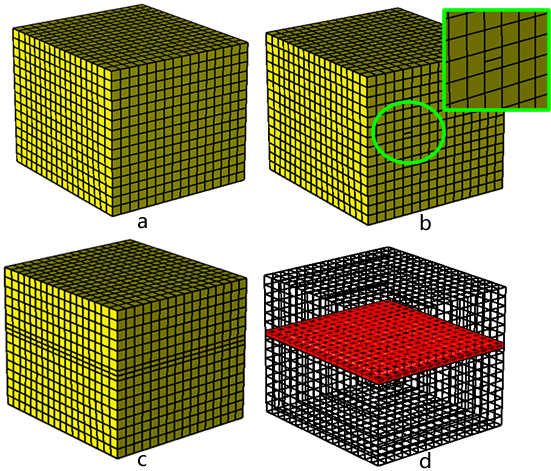
\includegraphics[width=9cm]{global_structure.png}
\caption{An example of local modification resulting in global change: (a) the original hex mesh; (b) local modification by adding a quad on the mesh boundary; (c) a circle of quads on the mesh boundary have to be added; (d) a set of hexahedra have to be added.}
\label{fig:global_structure}
\end{center}
\end{figure}

More specifically, starting from one mesh edge, we recursively get all its topologically parallel mesh edges. All of these mesh edges along with the adjacent hex define a sheet. In addition to its primal representation as a composition of vertices, edges, faces and hexahedra, a hex mesh can also be seen as a set of intersecting sheets, known as Spatial Twisted Continuum\cite{Murdoch:1997fy}.

Therefore, as a set of operations that directly and effectively deal with the sheets, sheet operations attract more and more attention in recent years. The most common sheet operations include pillowing\cite{Mitchell:1995wa}, dicing\cite{melander1997generation}, column collapse\cite{Staten:2009bo}, sheet extraction\cite{Staten:2009bo,Borden:2002hs} and sheet inflation\cite{Staten:2009bo,Ledoux:2009jz,staten2010sheet}.

\begin{figure}[htbp]
\begin{center}
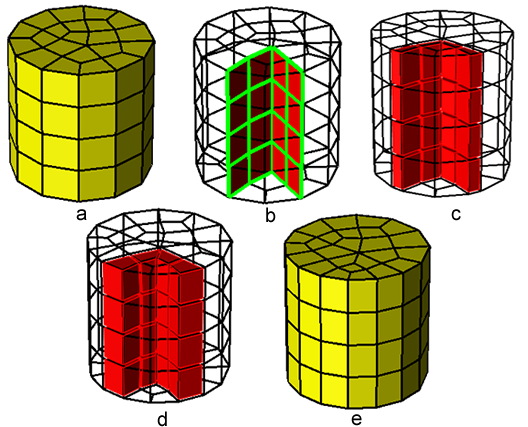
\includegraphics[width=8cm]{sheet_inflation.png}
\caption{The procedures of sheet inflation: (a) the hex mesh before sheet inflation; (b) the quad set for sheet inflation; (c) the new sheet is created by inflating the quad set; (d) the new sheet is created; (e) the hex mesh after sheet inflation.}
\label{fig:sheet_inflation}
\end{center}
\end{figure}

Sheet inflation takes a continuous quad set as input and generates a new sheet by inflating the quad set. The process of the sheet inflation is illustrated in Fig. \ref{fig:sheet_inflation}. This continuous quad set (Fig. \ref{fig:sheet_inflation}(b)) is called the quad set for sheet inflation (or quad set if not ambiguous in the context) which is provided by other procedures or specified directly by the user. Sheet inflation duplicates the nodes, edges, and quads on the quadset (Fig. \ref{fig:sheet_inflation}(b)) and then forms new hexahdedra by connecting the nodes in the quad set to their corresponding duplicates (Fig. \ref{fig:sheet_inflation}(c) and Fig. \ref{fig:sheet_inflation}(d)). The process of the sheet inflation shows that the quad set is critical for sheet inflation because it determines the position, shape and topology of the sheet to be generated by the sheet inflation. And compared with pillowing, sheet inflation is more flexible and versatile, having the potential ability to create any kind of sheets, provided that a suitable quad set can be determined. Therefore sheet inflation can be used to support various hex mesh modification.

Sheet inflation is a flexible and versatile sheet operation that can create various and complex sheets, and thus it can be utilized to effectively support many hex mesh modification scenarios. One common scenario is to use sheet inflation to locally change the mesh topology, especially the boundary topology of a hex mesh. In this scenario, new sheets usually need to be created to satisfy certain constraints like at the specified position within a delimited region. As the quad set plays a key role for sheet inflation, the main difficulty to achieve this is how to construct a qualified quad set under the given constraints. In practice, these constraints are normally specified by a set of boundary edges and a set of hexahedra. The former determines the positions where the new sheet should appear on the mesh boundary, and the latter delimits the region where the new sheet belongs to.

Figure \ref{fig:intro_high_val} shows an example where such constrained sheet inflation is required. In this example, the hex mesh (Fig. \ref{fig:intro_high_val}(a)) contains one boundary node whose valence is 6 and it is undesirable. As shown in Fig. \ref{fig:intro_high_val}(b), this high valence can be reduced by splitting the node into two nodes with lower valences, and a constrained sheet inflation can be used to achieve this. Specifically, two mesh edges adjacent to the high-valence node are selected as the position constraint of the new sheet (Fig. \ref{fig:intro_high_val_whole}(a)) first, then a quad set is constructed (Fig. \ref{fig:intro_high_val_whole}(b)), finally the new sheet is inflated based on the quad set (Fig. \ref{fig:intro_high_val_whole}(c))). The result is shown in Fig. \ref{fig:intro_high_val_whole}(e).

\begin{figure}[htbp]
\begin{center}
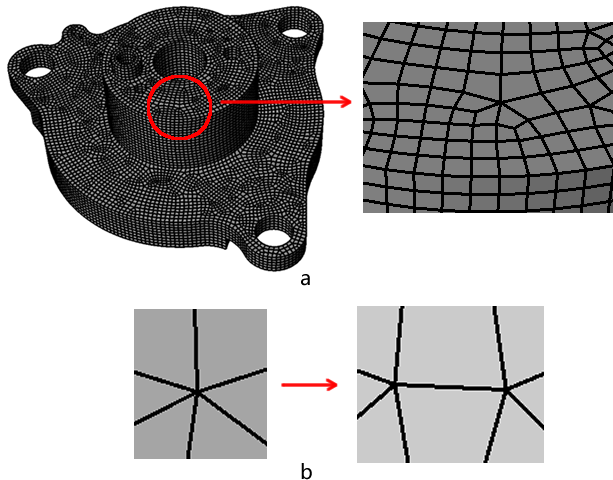
\includegraphics[width=8.5cm]{intro_high_val.png}
\caption{An example where boundary modification is required: (a) the hex mesh with a high-valence node; (b) the high valence is reduced by splitting the node into two nodes.}
\label{fig:intro_high_val}
\end{center}
\end{figure}

\begin{figure*}[htbp]
\begin{center}
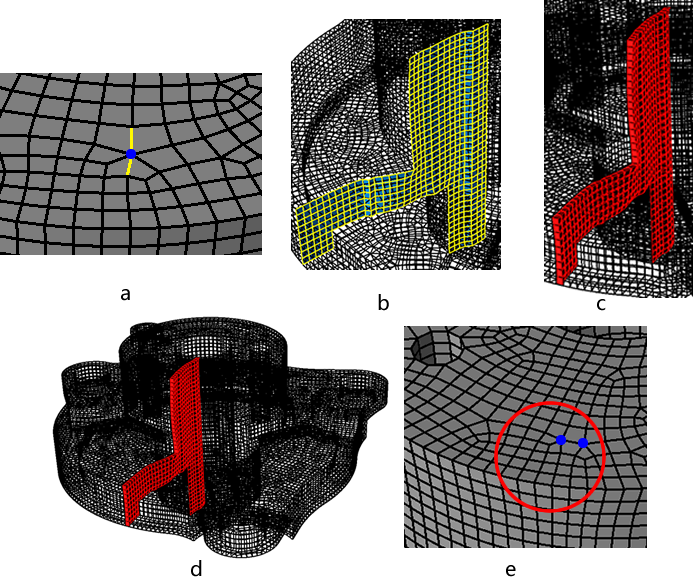
\includegraphics[width=12cm]{intro_high_val_whole.png}
\caption{Reducing high valence by non-localized sheet inflation : (a) selected mesh edges where new sheet needs inflating; (b) the quad set for sheet inflation without local consideration; (c) the new sheet; (d) the new sheet (from the global perspective); (e) the high valence is reduced.}
\label{fig:intro_high_val_whole}
\end{center}
\end{figure*}

Without region constraints being specified, the quad set may spread uncontrollably through the hex mesh, e.g. the quad set in Fig. \ref{fig:intro_high_val_whole}(b). Inflating quad sets like this will impact almost the whole mesh. To localize the sheet inflation, region constraints need specifying by a set of hexahedra (yellow in Fig. \ref{fig:intro_high_val_localized_inf}(a)). The quad set is then constructed within that delimited region (Fig. \ref{fig:intro_high_val_localized_inf}(b)). Compared to Fig. \ref{fig:intro_high_val_whole}(d), the localized sheet inflation will impact only a limited part of the hex mesh as shown in Fig. \ref{fig:intro_high_val_localized_inf}(d).

\begin{figure*}[htbp]
\begin{center}
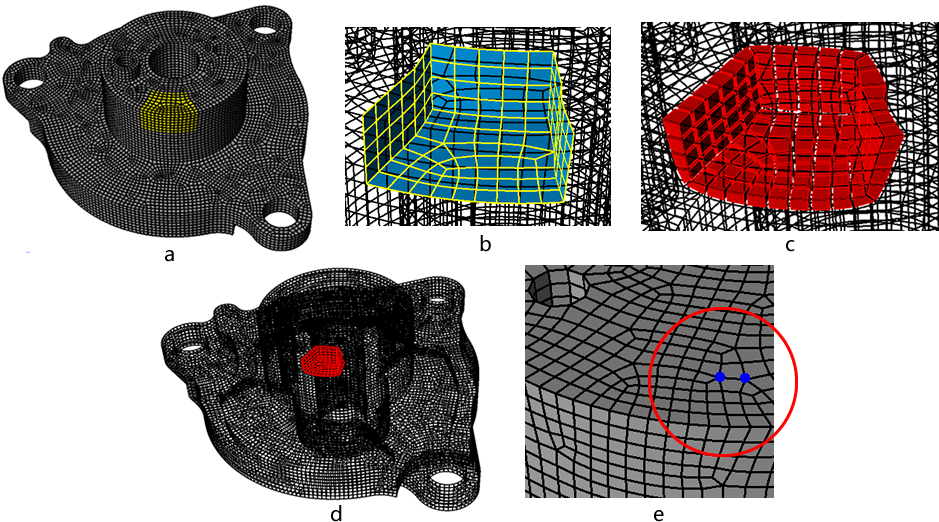
\includegraphics[width=15cm]{intro_high_val_localized_inf.png}
\caption{Reducing high valence by localized sheet inflation : (a) delimited region specified by a set of hex (yellow); (b) the localized quad set for sheet inflation; (c) the new sheet; (d) the new sheet is localized to the whole mesh; (e) the high valence is improved.}
\label{fig:intro_high_val_localized_inf}
\end{center}
\end{figure*}

In recognizing the importance of sheet inflation, many researchers have been investigating algorithms for decades and have achieved great progress. Mitchell et al. proposed the Pillowing algorithm to deal with the doublet problem\cite{Mitchell:1995wa}.  Its simplicity and effectiveness makes Pillowing prevalent in mesh modification, especially in mesh quality improvement. Although it can be adapted to satisfy simple constraints, Pillowing lacks the ability to generate complex sheets such as self-intersecting sheets.

Suzuki et al. introduced a method to construct interior sheet surfaces when the boundary dual cycles are given\cite{Suzuki:2010hn}. They used this method to first construct dual structures and then deduce the primal hex meshes from these dual structures. While in the paper they illustrated the topological structures of sheet surfaces in the dual space, particularly self-intersecting sheet surfaces, they didn't mention how to determine the quad set and generate the corresponding sheets on the primal hex mesh.

Staten et al. proposed the General Sheet Inflation method which explained in detail how to do sheet inflation on hex meshes when boundary mesh edges are specified\cite{Staten:2009bo}. This method can create normal, self-touching and self-intersecting sheets. However, Staten provides no details on how construct quad sets.  While his theory supports self-intersecting and self-touching sheets, it is not clear whether his algorithm can generate the required quad sets.

Sheet inflation is an enhanced and more general version of the classic pillowing. Pillowing actually can be seen as a special form of sheet inflation whose quad set is determined by the shared quad set between the shrinking set and the rest of the mesh.

Chen et al. proposed a new approach to inflate sheets when conducting mesh matching on complex interfaces\cite{Chen:2015kf}. This method first constructs the boundary loop of the quad set, and then determines the interior quad set. Although it can locally generate self-intersecting sheets under constraints, it allows the sheets to self-intersect no more than once. Meanwhile, the optimization method it applies on quad set cannot guarantee the quality improvement.

Despite these achievements, to inflate complex sheets under various constraints, especially to generate self-intersecting sheets within a local region, is still very difficult. Furthermore, how to assure the mesh quality for complex sheet inflation is also a challenging problem. Here it should be pointed out that in many situations it is imperative to locally create self-intersecting sheets. For the example in Fig. \ref{fig:intro_int_required}(a), where a node's valence is 7, splitting method shown in Fig. \ref{fig:intro_high_val}(b) can not effectively reduce the high valence since the valence of one new node is still 6 (Fig. \ref{fig:intro_int_required}(b)). Thus, instead of selecting two adjacent edges, four adjacent edges need to be selected and the node needs to be split into four nodes as shown in Fig. \ref{fig:intro_int_required}(c), which requires a self-intersecting sheet be generated. Since the edge valences (the number of the quads that are adjacent to the edge) have significant impact on the quality of quad mesh and hex mesh\cite{Staten2010d}, we use the irregular degrees (the edge's valence variance from a regular edge) of the quad set\cite{Chen:2015kf} to measure its quality in this work.

In this paper we propose a new approach to achieving complex sheet inflation by providing a new method of constructing complex quad sets. For a quad set, all its mesh edges on the hex mesh boundary form a loop/loops, called the quad set's boundary loop/loops. We first determine the boundary loop and utilize the max-flow-min-cut algorithm\cite{lawler20014} to construct an initial quad set that fulfills all the constraints. We then apply a chord-based optimization method to improve the quality of the quad set and thus the mesh quality after sheet inflation is guaranteed.

\begin{figure}[htbp]
\begin{center}
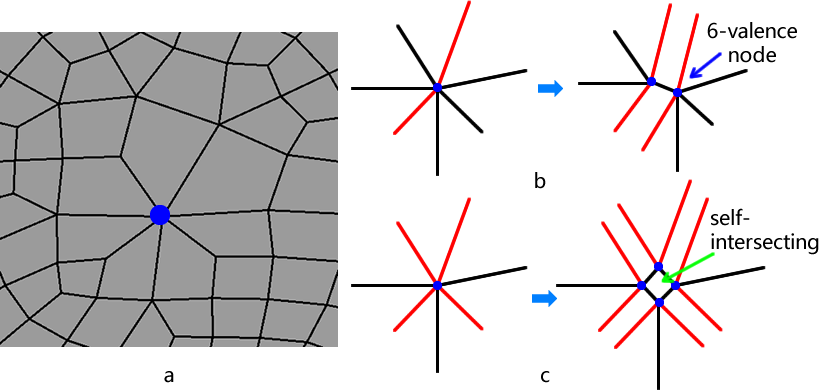
\includegraphics[width=8.5cm]{intro_int_required.png}
\caption{An example when a self-intersecting sheet is required to be generated: (a) the hex mesh with a high-valence node; (b) there is still a 6-valence node after splitting the node into two nodes; (c) the high valence is reduced by splitting the node into four nodes.}
\label{fig:intro_int_required}
\end{center}
\end{figure}

The rest of this paper is organized as below: we will show the outline of the approach in the second chapter, explain the procedures of constructing the boundary loops of quad sets in the third chapter, provide the details of the determination and optimization of the initial quad set in the fourth and fifth chapters respectively, and then give some results in the sixth chapter and list conclusions and future work in the last chapter.

%%%%%%%%%%%%%%%%%%%%%%%%%%%%%%%%%%%%%%%%%%%%%%%%%%%%%%%%%%%%%%%%%%%%%%%%%%
\section{Overview of the Approach}
\label{sec:algo_overview}

In this paper, an approach is proposed to achieving complex sheet inflation under various constraints while maximizing mesh quality. It takes a set of boundary mesh edges and a set of hexahedra as input. The edges specify the boundary position where the new sheet should appear. The hexahedra set refers to the delimited region where the new sheet belongs to. It is specified by the user and used to achieve local sheet inflation. Under these constraints, it constructs a qualified quad set and then creates the new sheet as output. To avoid the difficulty of determining a qualified inflatable quad set directly, our approach involves three major steps: (1) determining the boundary loops for the quad set that satisfy the boundary constraints; (2) constructing the initial quad set based on the boundary loops; (3) optimizing the initial quad set. Figure \ref{fig:overview} shows the overview of our approach.


\begin{figure*}[htbp]
\begin{center}
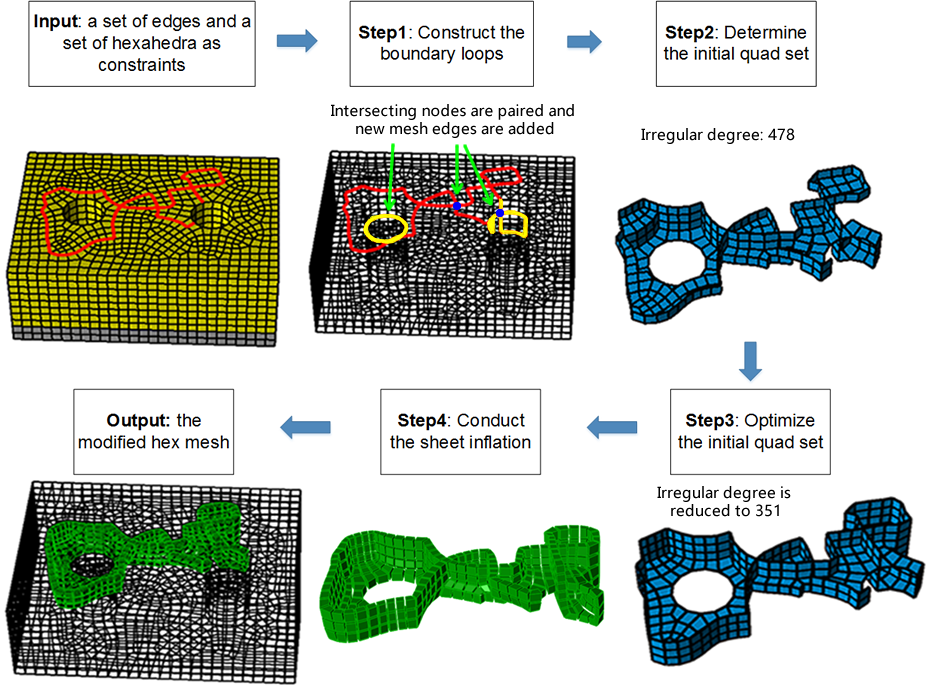
\includegraphics[width=16cm]{overview2.png}
\caption{Flowchart of the optimized complex sheet inflation.}
\label{fig:overview}
\end{center}
\end{figure*}

Our approach needs to solve two critical problems. The first problem is how to construct the valid boundary loop and initial quad set satisfying various boundary constraints. Boundary constraints specified by the user can be either a loop or just a set of edges, and can be non-self-intersecting or intersecting itself more than once. The second problem is how to effectively optimize the initial quad set when a global optimal result can hardly be reached.

To solve these two problems, our basic ideas are:
\begin{enumerate}
  \item We use path searching and max-flow-min-cut algorithms to construct the valid boundary loop and initial quad set that meet the various boundary constraints. In accordance with the inherent characteristics of valid boundary loops and quad sets, loops can be formed by the path searching algorithm if the boundary constraints are not loops, and intersecting lines on the quad set can also be determined by the path searching algorithm. The valid boundary loop and initial quad set can be effectively determined by the max-flow-min-cut algorithm due to the fact that the determination of these structures on the mesh is analogous to finding a cut set on a graph;
  \item We optimize the initial quad set by optimizing its chords, which are the dual structures of the quad set. The chords are more global than individual edges while less constrained than the whole quad set. By optimizing the chords, we can effectively improve the quality of the quad set while avoiding the difficulty in optimizing the quad set as a whole.
\end{enumerate}

In the following sections specific details of the major steps are provided.

%%%%%%%%%%%%%%%%%%%%%%%%%%%%%%%%%%%%%%%%%%%%%%%%%%%%%%%%%%%%%%%%%%%%%%%%%%
\section{Determination of the Boundary Loops}
\label{sec:det_bound_loops}
It is quite difficult to find a qualified quad set satisfying all the constraints directly. The quad set's boundary loop is constructed first. This section first discusses the characteristics of valid boundary loops and quad sets, and then presents the method to construct a valid boundary loop under the boundary constraints.

By observation of the structures of valid quad sets and the process of sheet inflation, an inflatable quad set and its boundary loop have two characteristics:

\begin{figure*}[htbp]
\begin{center}
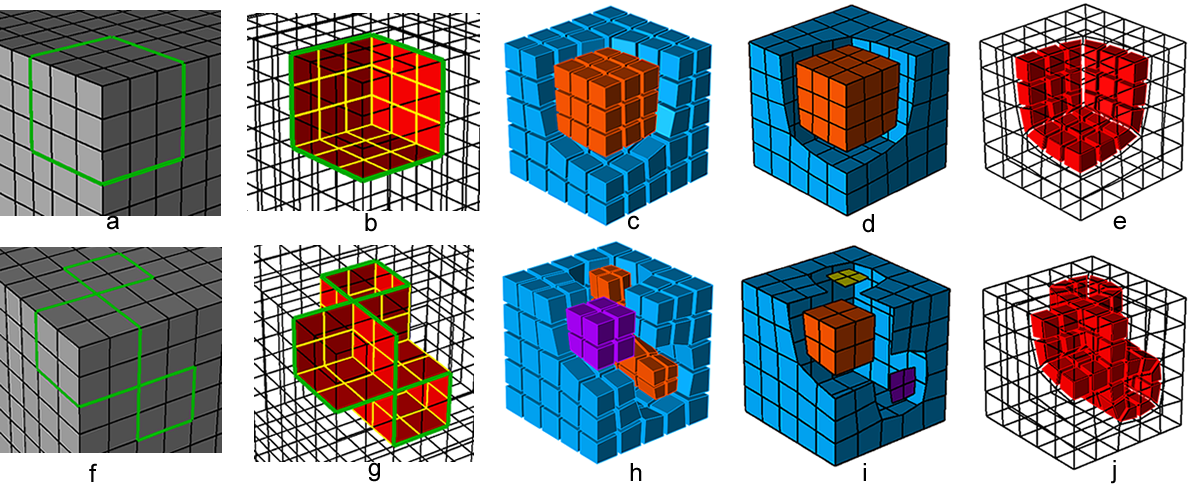
\includegraphics[width=15cm]{compo_loop_prop.png}
\caption{Characteristics of valid boundary loops: (a) a non-self-intersecting boundary loop; (b) the non-self-intersecting quad set; (c) two hex sets separated by the quad set; (d) two boundary quad sets separated by the boundary loop; (e) the new non-self-intersecting sheet; (f) a self-intersecting boundary loop; (g) the self-intersecting quad set; (h) three hex sets separated by the quad set; (i) four boundary quad sets separated by the boundary loop; (j) the new self-intersecting sheet.}
\label{fig:loop_prop}
\end{center}
\end{figure*}

\begin{enumerate}
\item An inflatable quad set separates its local hex set into $2+N$ subsets, where $N$ stands for how many times the quad set intersects itself. For example, the non-self-intersecting quad set in Fig. \ref{fig:loop_prop}(b) separates the local hex set into two parts (Fig. \ref{fig:loop_prop}(c)). The self-intersecting quad set in Fig. \ref{fig:loop_prop}(g) separates the local hex set into 3 subsets (Fig. \ref{fig:loop_prop}h). Meanwhile, the boundary loop of the quad set separates the boundary of the local hex set into $2+n$ subsets, where $n$ is the number of self-intersecting nodes on the boundary loop. The non-self-intersecting boundary loop in Fig. \ref{fig:loop_prop}(a) separates the boundary of the local hex set into two subsets (Fig. \ref{fig:loop_prop}(d)), and the self-intersecting boundary loop in Fig. \ref{fig:loop_prop}(f) separates the boundary of the local hex set into 4 subsets (Fig. \ref{fig:loop_prop}(i)).

\item Intersecting nodes on the boundary loop can be grouped into pairs. An intersecting line on the quad set can be found between two nodes in each pair.
\end{enumerate}

The first characteristic, which is also called local separation, means that the quad set separates the hex set that is local to the quad set into a certain number of hex subsets. It is necessary for a quad set to be inflatable, because the sheet inflation operation is actually done by separating the hex subsets and filling the gaps with new hexahedra, as shown in Fig. \ref{fig:loop_prop}(c), Fig. \ref{fig:loop_prop}(e), Fig. \ref{fig:loop_prop}h and Fig. \ref{fig:loop_prop}(j). It also indicates that the boundary loops must be closed otherwise new hexahedra on the mesh boundary will not be correctly created. The second characteristic also indicates that each intersecting node on the boundary loop needs to be paired with another intersecting node in order to determine an intersecting line, which means there should be an even number of intersecting nodes on the boundary loop. This also indicates that a boundary with loop with an odd number of intersecting nodes is invalid for constructing a quad set for sheet inflation.

\begin{figure}[htbp]
\begin{center}
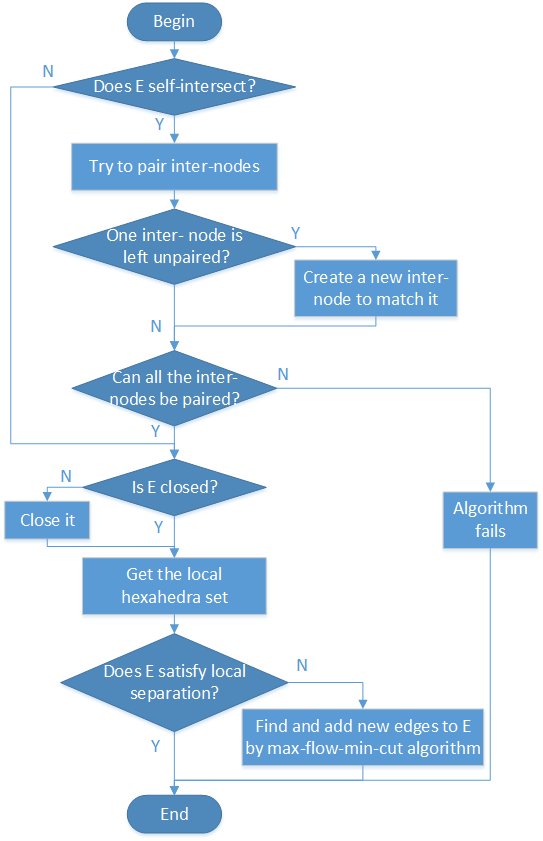
\includegraphics[width=8cm]{flow_det_loop.png}
\caption{Flowchart of the determination of boundary loops.}
\label{fig:flow_det_loop}
\end{center}
\end{figure}

Based on the above analysis, we check whether the specified constraint edges are eligible to be a valid boundary loop. If not, we use the path searching algorithm and max-flow-min-cut algorithm to determine a valid boundary loop. The flowchart of the determination of boundary loops is shown in Fig. \ref{fig:flow_det_loop}. Note that $E$ in Fig. \ref{fig:flow_det_loop} denotes the constraint mesh edges specified by the user. The rest of this section will provide detailed description about the method of the determination of boundary loops.

%%%%%%%%%%%%%%%%%%%%%%%%%%%%%%%%%%%%%%%%
\subsection{Pairing Intersecting Nodes}
\label{sec:int_pt_pair}
For self-intersecting quad sets, the intersecting line plays a very important role in defining the structures of the quad sets, which is a piecewise continuous set of edges interior to the hex mesh connecting a pair of intersecting nodes. Therefore, the intersecting nodes on the boundary lines need to be paired in order to construct the intersecting line between each pair of intersecting nodes.When there are more than two intersecting nodes, improper pairing of intersecting nodes can result in non-orientable surface with very poor quality or even no surface at all\cite{Suzuki:2010hn}. Based on the observation about the structures of quadrilateral sets, we introduce two types of local intersecting structures that can be used to effectively pair intersecting nodes. By recursively searching these two types of local intersecting structures from the input boundary mesh edges, properly pairing of intersecting nodes can be achieved.

\begin{figure*}[htbp]
\begin{center}
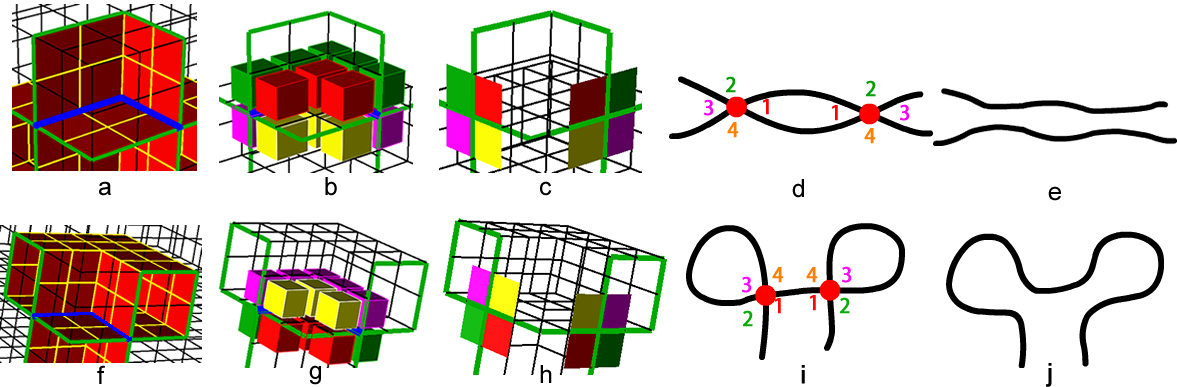
\includegraphics[width=17cm]{pair_patterns.png}
\caption{Two types of local intersecting structure for pairing intersecting nodes: (a) the 1st local intersecting quad subset; (b) int-4-hex-sets around the 1st local intersecting quad subset; (c) the 1st local intersecting structure of the boundary loop; (d) the pairing information of the 1st local intersecting structure; (e) the 1st local intersecting structure is resolved for recursive searching; (f) the 2nd local intersecting quad subset; (g) int-4-hex-sets around the 2nd local intersecting the quad subset; (h) the 2nd local intersecting structure of the boundary loop; (i) the pairing information of the 2nd local intersecting structure; (j) the 2nd local intersecting structure is resolved for recursive searching.}
\label{fig:int_pair_tpl}
\end{center}
\end{figure*}

On various intersecting quad sets, two types of local intersecting quad subsets are commonly observed which are shown in Fig. \ref{fig:int_pair_tpl}(a) and Fig. \ref{fig:int_pair_tpl}(f). These two types of quad subsets both have one intersecting line and two intersecting nodes on their boundary loops. The topological structures of their boundary loops are shown in Fig. \ref{fig:int_pair_tpl}(d) and Fig. \ref{fig:int_pair_tpl}(i). Conversely, if a local intersecting structure of the mesh edges is found to share the same topology with that shown in Fig. \ref{fig:int_pair_tpl}(d) or Fig. \ref{fig:int_pair_tpl}(i), there should be a corresponding local intersecting quad subset. Hence, it is reasonable to pair the two intersecting nodes on this local part of the mesh edges, which will not result in the improper pairing mentioned in \cite{Suzuki:2010hn}.

To recursively find pairs of intersecting nodes, the local topological structures are modified accordingly as shown in Fig. \ref{fig:int_pair_tpl}(e) and Fig. \ref{fig:int_pair_tpl}(j). Currently, we treat these two local intersecting structures equally and use a depth-first strategy to search and handle the two types of local intersecting structures, which means if we find either local intersecting structure, we pair its two intersecting nodes involved in the structure and modify it at once until no more intersecting nodes can be paired.

Some structures near the intersecting lines or intersecting nodes are very important for determining the quad set later. The hexahedra adjacent to the intersecting lines are separated into four subsets by the local structures of quad sets, as shown in Fig. \ref{fig:int_pair_tpl}(b) and Fig. \ref{fig:int_pair_tpl}(g). These hex subsets are called int-4-hex-sets of the intersecting line. The associated local structures of boundary loops are shown in Fig. \ref{fig:int_pair_tpl}(c) and Fig. \ref{fig:int_pair_tpl}(h). The quads of same color mean they are adjacent to the same int-4-hex-set. The numbers in different colors on the two local intersecting structures in Fig. \ref{fig:int_pair_tpl}(d) and Fig. \ref{fig:int_pair_tpl}(i) indicate the corresponding int-4-hex-sets.

Two examples in Fig. \ref{fig:pair_int_exams} are presented to explain how to pair intersecting nodes by searching these two local intersecting structures.

\begin{figure}[htbp]
\begin{center}
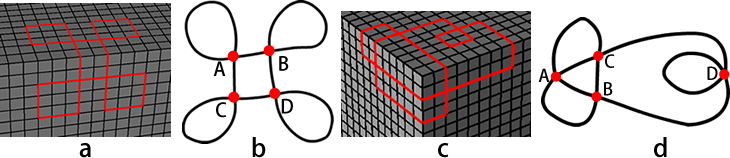
\includegraphics[width=8.5cm]{pmatchexams.png}
\caption{Two examples of pairing intersecting nodes: (a) the boundary loop of the 1st example; (b) the topological structure of the boundary loop of the 1st example; (c) the boundary loop of the 2nd example; (d) the topological structure of the boundary loop of the 2nd example.}
\label{fig:pair_int_exams}
\end{center}
\end{figure}

The pairing process for the 1st example is shown in Fig. \ref{fig:pair_int_exam1_proc}. The intersecting nodes $A$ and $B$ are first paired according to the 1st local intersecting structure. After topological structure is modified, $C$ and $D$ are also paired according the 1st local intersecting structure.

\begin{figure}[htbp]
\begin{center}
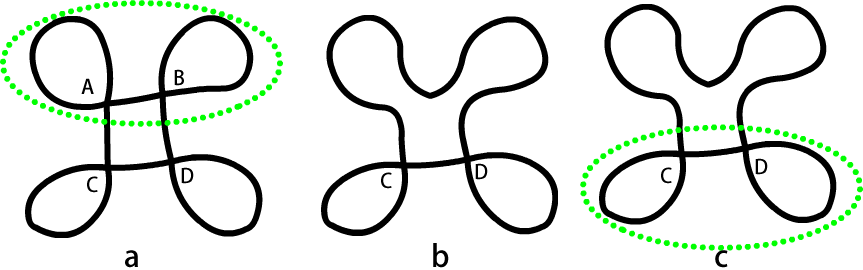
\includegraphics[width=8cm]{pmexam1step.png}
\caption{The pairing process of the 1st example: (a) node $A$ and $B$ are paired; (b) node $A$ and $B$ are resolved; (c) node $C$ and $D$ are paired.}
\label{fig:pair_int_exam1_proc}
\end{center}
\end{figure}

The pairing process for the 2nd example is shown in Fig. \ref{fig:pair_int_exam2_proc}. The intersecting nodes $A$ and $B$ are first paired according to the 2nd local intersecting structure. After topological structure is modified, the nodes $C$ and $D$ are paired based on the 1st local intersecting structure.

\begin{figure}[htbp]
\begin{center}
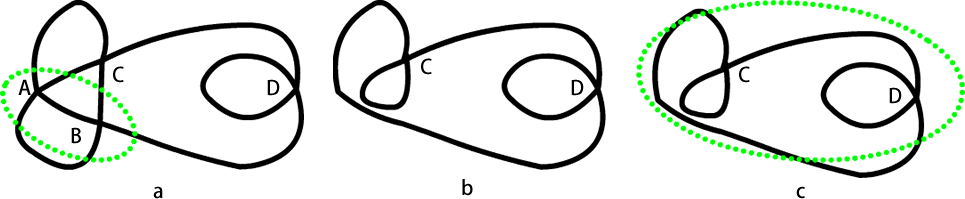
\includegraphics[width=8cm]{pmexam2step.png}
\caption{The pairing process of the 2nd example: (a) node $A$ and $B$ are paired; (b) node $A$ and $B$ are resolved; (c) point $C$ and $D$ are paired.}
\label{fig:pair_int_exam2_proc}
\end{center}
\end{figure}

After recursively searching these two local intersecting structures, if there is still one intersecting node left unpaired, we need to create a new intersecting node at a appropriate position in order to pair these two intersecting node according to the local intersecting structures. The creation can be automatic based on the topological information provided by the two types of local intersecting structures.

For example, in Fig. \ref{fig:create_int_node}(a), the intersecting node $A$ is unpaired. Since a substructure of the 1st intersecting structure can be found in current mesh edges, which contains a closed circle with a single intersecting node, the 1st intersecting structure is used to help us create the second intersecting node. First, we choose either end nodes on the current mesh edges, $v$ in Fig. \ref{fig:create_int_node}(a) for instance. Second, from $v$ we search for a suitable mesh node to be the second intersecting node $B$ which should meet two requirements: 1) its node valence should be no less than 4 in order to be an intersecting node; 2) the distance between $B$ and $v$ should be relatively equal to $len$ (length from $A$ to $v$ as shown in Fig. \ref{fig:create_int_node}(b)) to make $B$ and $A$ symmetrical to $v$ which usually enhances the mesh quality. The second intersecting node $B$ is determined in Fig. \ref{fig:create_int_node}(b). Third, according to the 1st local intersecting structure, the substructure at $B$ is constructed (Fig. \ref{fig:create_int_node}(c)). At last, to achieve better symmetry, we extend the edge circle adjacent to $B$ to the extent that encloses a similar number of quads as the circle adjacent to $A$ as shown in Fig. \ref{fig:create_int_node}(d).

\begin{figure}[htbp]
\begin{center}
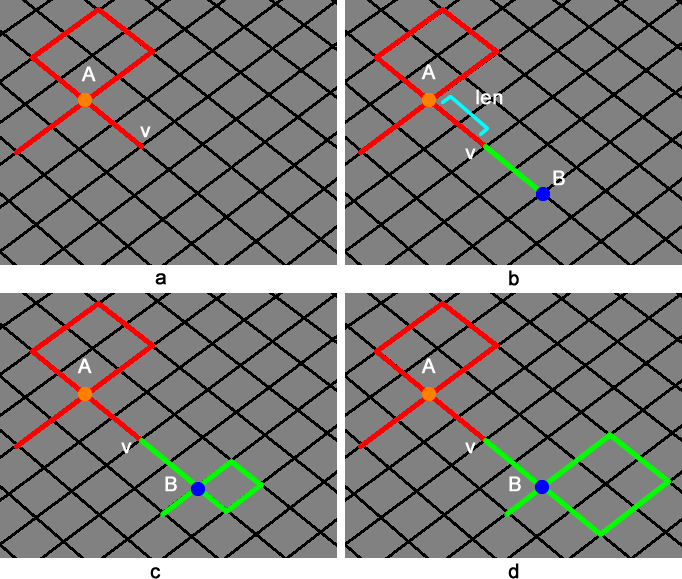
\includegraphics[width=8.7cm]{create_int_node.png}
\caption{Handling of the situation when single intersecting node is unpaired: (a) intersecting node $A$ is unpaired; (b) the new intersecting node $B$ is determined; (c) the substructure adjacent to $B$ is constructed; (d) the edge circle adjacent to $B$ is expanded according to the size of the edge circle adjacent to $A$.}
\label{fig:create_int_node}
\end{center}
\end{figure}

Our algorithm would fail if some intersecting nodes are unable to be paired according to the two local intersecting structures. These boundary loops usually determine non-orientable quad sets\cite{Suzuki:2010hn} which will largely degenerate the mesh quality after sheet inflation. Therefore we do not handle such kind of boundary loops in this paper.

%%%%%%%%%%%%%%%%%%%%%%%%%%%%%%%%%%%%%%%%
\subsection{Forming Closed Boundary Loops}
\label{sec:close_bound_loop}
The ability to do local separation requires the constraint edges to form closed loops. Sometimes the constraint edges, which are specified by the user according to specific mesh modification requirements, may not be closed loops. When this happens, we need to close the constraint edges by adding new edges on the mesh boundary. This is done by connecting the dangling edges on the constraint edges using the A* path searching algorithm\cite{hart1968formal}.

A* path searching is a one-source-one-target path searching algorithm which runs very efficiently. It is an extension of the Dijkstra's algorithm\cite{Dijkstra1959A}. The formalization of A* algorithm is shown in Equ. \ref{equ:a_star}. Here, $g(n)$ is the known cost of getting from the initial node to $n$; this value is tracked by the algorithm. $h(n)$ is a heuristic estimate of the cost to get from $n$ to the target node. For the algorithm to find the actual shortest path, the heuristic function $h(n)$ should never overestimate the actual cost to get to the target node.

\begin{equation}
\label{equ:a_star}
f(n)=g(n) + h(n)
\end{equation}

Given two boundary mesh edges $e_1$ and $e_2$ and their common mesh node $v$, $e_1$ and $e_2$ separate $v$'s adjacent quads into to quad subsets $Q_1$ and $Q_2$. The turning angle in this paper is the quad number variance between these two quad subsets, which can be calculated by Equ. \ref{equ:turn_angle} where $\left \| Q_1 \right \|$ and $\left \| Q_2 \right \|$ stand for the number of quads in $Q_1$ and $Q_2$ respectively.

\begin{equation}
\label{equ:turn_angle}
ta(e_1,e_2)=\begin{Vmatrix}
\left \| Q_1 \right \| - \left \| Q_2 \right \|
\end{Vmatrix}
\end{equation}

For example, in Fig. \ref{fig:turning_angle}(a), $Q_1$ and $Q_2$ contain 1 and 3 quads respectively. So $ta(e_1,e_2)=2$. In Fig. \ref{fig:turning_angle}(b), $Q_1$ and $Q_2$ both contain 2 quads. So $ta(e_1,e_2)=0$.

\begin{figure}[htbp]
\begin{center}
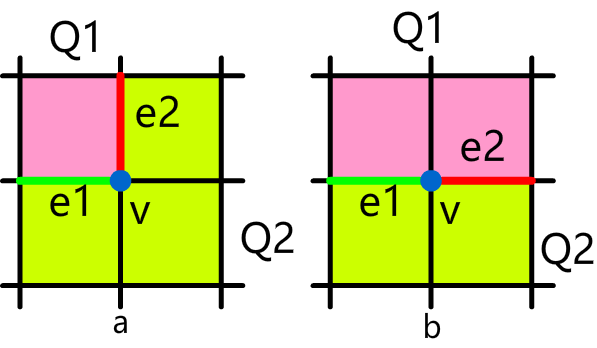
\includegraphics[width=7cm]{turning_angle.png}
\caption{Turning angles between two boundary mesh edges: (a) the two edges separate the $v$'s adjacent to two quad subsets and $\left \| Q_1 \right \|=1$ and $\left \| Q_2 \right \|=3$; (b) the two edges separate the $v$'s adjacent to two quad subsets and $\left \| Q_1 \right \|$ and $\left \| Q_2 \right \|$ are both 2.}
\label{fig:turning_angle}
\end{center}
\end{figure}

When applying A* algorithm, in addition to considering the count of mesh edges on the path, we also take the angles between adjacent edges on the path into consideration. This is necessary because if the turning angles are large, the mesh quality, especially the boundary mesh quality, will degenerate. Therefore, suppose the current mesh edges are $E$, the determined part in A* algorithm can be calculated using Equ. \ref{equ:det_part} where $\left \| E \right \|$ stands for the number of edges in $E$. The weight $\rho $ controls the magnitude of how the turning angle impacts on the searching result. Usually $\rho =1$ is feasible.

\begin{equation}
\label{equ:det_part}
g(E) = \rho * \sum ta(e) + \left \| E \right \|, e \in E
\end{equation}

For the heuristic part of A*, we use a breadth-first strategy to estimate at least how many mesh edges are needed to be traversed from current node to the target node. Since the breadth-first estimation only takes the number of traversed edges into consideration, it meets the requirement in A* algorithm that $h(n)$ should never overestimate the actual cost to get to the target node. For example, after conducting a breadth-first iteration, the minimum numbers of mesh edges that are needed to be traversed from a given mesh node to $v_1$ are shown in Fig. \ref{fig:A_start_estimation}(a). Therefore $h(v_2)=2$ and $h(v_3)=4$.

\begin{figure}[htbp]
\begin{center}
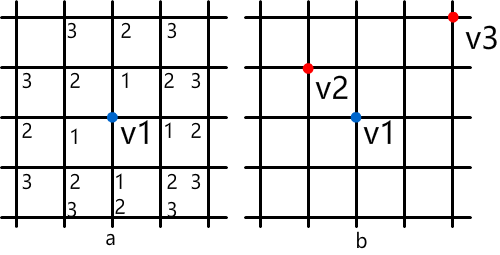
\includegraphics[width=7cm]{A_start_estimation.png}
\caption{Estimation for the heuristic distance between two nodes: (a) the minimum distances are calculated by using a breadth-first iteration; (b) the heuristic distances of $v_2$ and $v_3$ regarding to $v_1$ are 2 and 4 respectively.}
\label{fig:A_start_estimation}
\end{center}
\end{figure}

Figure \ref{fig:close_loop}(b) shows the result when the angles between adjacent edges are not considered, and Fig. \ref{fig:close_loop}(c) shows a better result when the angles are taken into consideration.

\begin{figure}[htbp]
\begin{center}
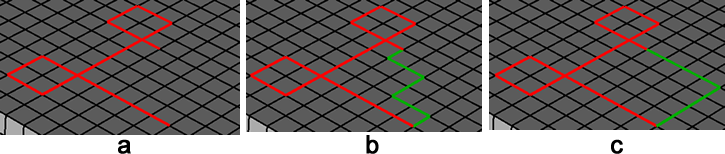
\includegraphics[width=9cm]{close_loop.png}
\caption{Closing the boundary loop: (a) the unclosed boundary loop; (b) new edges determined by A* algorithm without considering the turning angles; (c) new edges determined by A* algorithm considering the turning angles.}
\label{fig:close_loop}
\end{center}
\end{figure}

%%%%%%%%%%%%%%%%%%%%%%%%%%%%%%%%%%%%%%%%
\subsection{Making the Boundary Loop Able to Do Local Separation}
\label{sec:local_separation}
After previous sections, the constraint edges specified by the user become a closed boundary loop with intersecting nodes being paired. According to the discussion in the beginning of Section \ref{sec:det_bound_loops}, a valid boundary loop should be able to do local separation. Sometimes the closed boundary loop may fail to do local separation due to the existence of through holes on the hex mesh. To fix that, we use the max-flow-min-cut algorithm to add necessary edges to the boundary loop to make it able to do local separation. Suppose the boundary loop is $E$, the algorithm flowchart is illustrated in Fig. \ref{fig:flow_local_sep}.

\begin{figure}[htbp]
\begin{center}
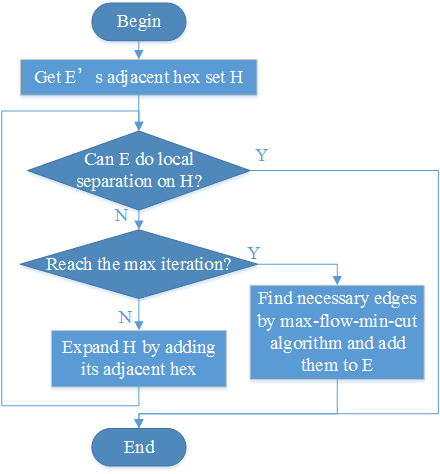
\includegraphics[width=7cm]{flow_local_separation.png}
\caption{Flowchart of the process of making the boundary loop able to do local separation.}
\label{fig:flow_local_sep}
\end{center}
\end{figure}

The following example illustrates the process. Figure \ref{fig:local_sep_exam}(a) shows the hex mesh containing a through hole and the boundary loop $E$ (red). To check whether $E$ is able to do local separation, we first get $E$'s adjacent hex set $H$ (Fig. \ref{fig:local_sep_exam}(b)) and iteratively add $H$'s adjacent hexahedra to $H$ and test whether the new boundary of $H$ can be separated by $E$ into two subsets before reaching the maximum iteration times (Fig. \ref{fig:local_sep_exam}(c)). However, $E$ is still unable to do local separation on $H$ since there are still only one quad set (blue in Fig. \ref{fig:local_sep_exam}(d)) on $H$'s boundary. Hence, we need to use the max-flow-min-cut algorithm to add other necessary mesh edges to $E$ to make it able to do local separation.

\begin{figure}[htbp]
\begin{center}
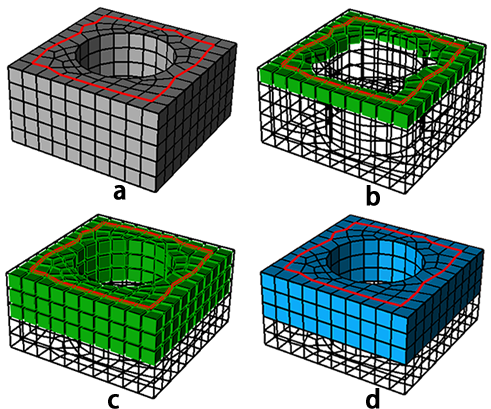
\includegraphics[width=6.5cm]{local_sep_exam.png}
\caption{An example of boundary loops that are unable to do local separation: (a) the boundary loop $E$; (b) $E$'s adjacent hexahedra $H$(green); (c) expand $H$ by iteratively adding its adjacent hexahedra; (d) $E$ still cannot separate $H$'s boundary into two subsets when reaching maximum expanding iteration times.}
\label{fig:local_sep_exam}
\end{center}
\end{figure}


Max-flow-min-cut algorithm is an effective and efficient algorithm to find the minimal cut set in a directed graph. On a directed graph with weighted edges, i.e. a flow graph, the maximum flow is the maximum amount of flow passing from the source (the $s$ node) to the sink (the $t$ node). And the minimum cut is the cut (a partition of the vertices of a graph into two disjoint subsets) no more intersecting nodes can be paired. The max-flow-min-cut theorem states that given a flow graph and $s$ and $t$ nodes, the max-flow equals the min-cut.

As shown in Fig. \ref{fig:max_flow_graph}(a), to use the max-flow-min-cut algorithm, a directed graph should be constructed with an $s$ node and a $t$ node, and the weights of the edges should also be set before calculation. The algorithm will find a minimal cut set that determines the max flow from $s$ to $t$.

If we take the boundary of $H$ as a graph where the nodes stand for a quad or a quad set and the edges stand for the adjacency relationship between the quads or quad sets, then to be able to do local separation is similar to find a cut set on this graph. Hence, the max-flow-min-cut algorithm can be used to help us to find necessary edges to make the boundary loop satisfy the local separation. Specifically, in this work, we use the Ford-Fulkeson\cite{ford1956maximal} method to efficiently compute the maximum flow in a flow graph.

To use the algorithm, we need to construct the directed graph at first, including constructing the $s$ and $t$ nodes and deciding the edges' weights. As the current boundary loop $E$ must be part of the final boundary loop, the two quad sets on its two sides just can be the $s$ and $t$ nodes as shown in Fig. \ref{fig:max_flow_graph}(b). Since all of the edges on the final boundary loop should be on the boundary of the hex mesh, the quads shared by $H$ and the rest of the hex mesh, which is shown as $Q_{in}$ in Fig. \ref{fig:max_flow_graph}(b), should be accordingly grouped into a single node in the graph to guarantee that $Q_{in}$ won't be separated by the min cut. Additionally, mesh edges whose adjacent quads are all boundary quads should not be added into the boundary loop because it usually results in poor mesh quality if the quad set for sheet inflation contains boundary quads. Hence we group the quads sharing these mesh edges into a single node. For example, $q_2$ and $q_3$ in Fig. \ref{fig:max_flow_graph}(c) are grouped into a single node.

After constructing the nodes, we assign weights to the graph edges according to how many mesh edges are shared by the two nodes. For example, $q_1$ in Fig. \ref{fig:max_flow_graph}(c) shares two edges with node $t$, so the weight of the directed edges in the graph between $q_1$ and $t$ is 2. There is one directed edge from $s$ node to each of its adjacent nodes. Similarly, for each of $t$'s adjacent nodes, there is one directed edge from this node to $t$. For each pair of adjacent nodes, if they are neither $s$ node nor $t$ node, there is a pair of opposite directed edges with the same weight between the two nodes.

The final directed graph is shown in Fig. \ref{fig:max_flow_graph}(d). After calculation, new edges are found as shown in Fig. \ref{fig:max_flow_graph}(e), and now $E$ is able to do local separation after adding these new edges as shown in  Fig. \ref{fig:max_flow_graph}(f).

\begin{figure}[htbp]
\begin{center}
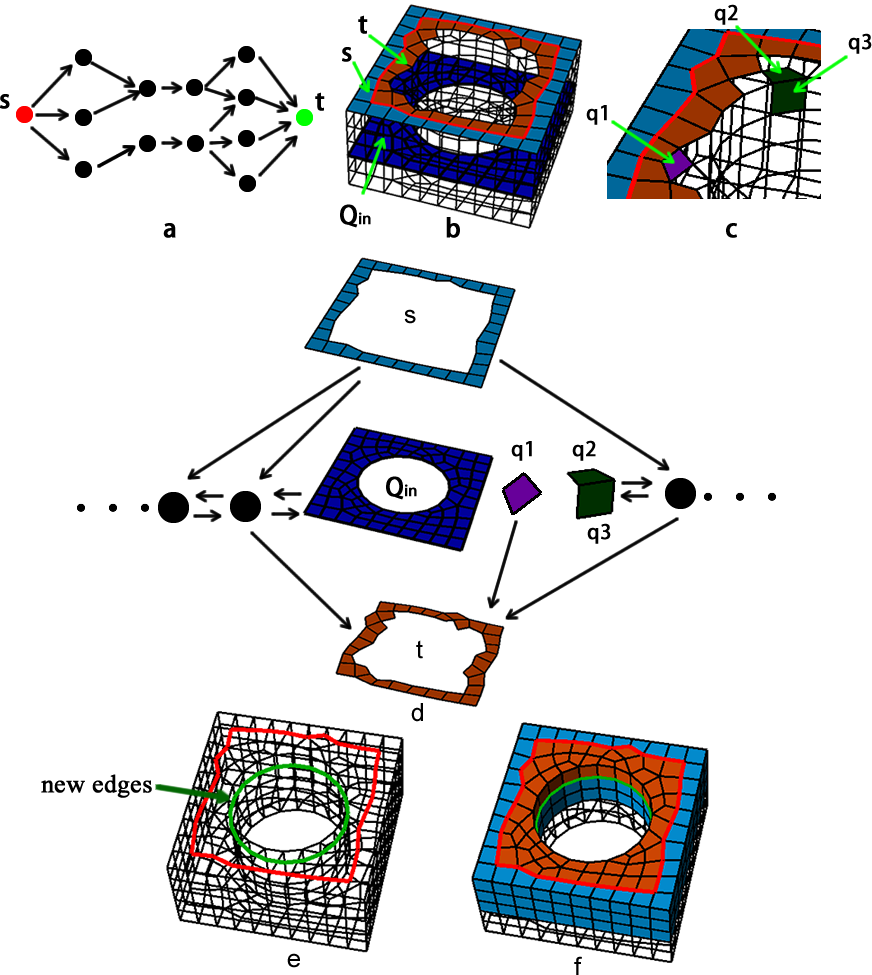
\includegraphics[width=9cm]{max_flow_graph.png}
\caption{Using max-flow-min-cut algorithm to find necessary edges for local separation: (a) directed graph used for ordinary max-flow-min-cut problem; (b) the quad sets on $E$'s two sides can be $s$ and $t$ nodes; (c) $q_1$ shares two edges with $t$, $q_2$ and $q_3$ share an edge on the geometric hard edge; (d) the directed graph for max-flow-min-cut algorithm; (e) new edges are found (green); (f) $E$ is able to do local separation after adding new edges.}
\label{fig:max_flow_graph}
\end{center}
\end{figure}

When a self-intersecting boundary loop is unable to do local separation, we also need to apply max-flow-min-cut algorithm to find necessary new edges to make it able to do local separation. The procedures are quite similar to non-self-intersecting boundary loop discussed previously. We treat a self-intersecting boundary loop as several non-self-intersecting boundary loops and handle each of them individually. The self-intersecting boundary loop in Fig. \ref{fig:int_loop_local_sep}(a) consists of three sub loops $loop_1$, $loop_2$ and $loop_3$. The local hex set is shown in Fig. \ref{fig:int_loop_local_sep}(b). Due to the existence of three through holes on the hex mesh, the boundary loop is unable to do local separation. After applying max-flow-min-cut algorithm to $loop_1$ and $loop_3$, new edges are found as shown in Fig. \ref{fig:int_loop_local_sep}(c).

\begin{figure}[htbp]
\begin{center}
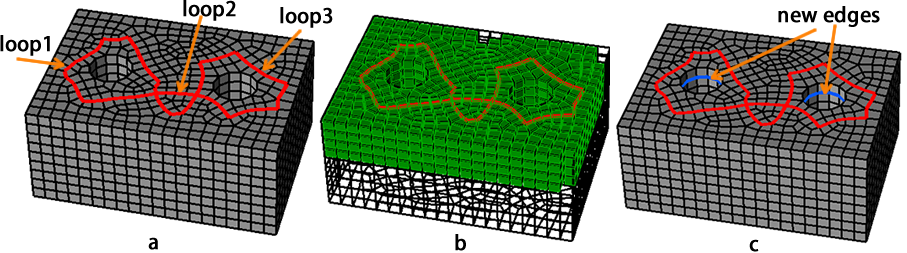
\includegraphics[width=9cm]{int_loop_local_sep.png}
\caption{Making self-intersecting boundary loop able to do local separation: (a) the self-intersecting boundary loop with three sub loops; (b) the local hex set; (c) new edges (blue) are found by using max-flow-min-cut algorithm.}
\label{fig:int_loop_local_sep}
\end{center}
\end{figure}

%%%%%%%%%%%%%%%%%%%%%%%%%%%%%%%%%%%%%%%%%%%%%%%%%%%%%%%%%%%%%%%%%%%%%%%%%%
\section{Determination of the Initial Quad Set}
\label{sec:det_quad_set}
This section provides specific details of the determination of the initial quad set based on the boundary loop. The intersecting lines are first constructed according to the pairing of the intersecting nodes. The initial quad set is then constructed using the max-flow-min-cut algorithm. Since the boundary loops satisfy the boundary constraints and the max-flow-min-cut algorithm is conducted within the local region specified by the user, the initial quad set fulfills all the constraints.

%%%%%%%%%%%%%%%%%%%%%%%%%%%%%%%%%%%%%%%%
\subsection{Determination of Intersecting Lines}
\label{sec:det_int_lines}
Intersecting lines, each of which connect a pair of intersecting nodes, are very important for defining the structures of self-intersecting quad sets. Before determining the initial quad set, we need to construct the intersecting lines first. In Section \ref{sec:int_pt_pair} the two local intersecting structures not only make two intersecting nodes be paired but also setup the corresponding relationships between the int-4-quad-sets of the two intersecting nodes. In this section, we use this information to construct the intersecting lines and the int-4-hex-sets of these intersecting lines.

The following example shows the process of constructing the intersecting line and its int-4-hex-sets. In Fig. \ref{fig:det_int_line}(a), the blue nodes are two intersecting nodes paired based on the 1st local intersecting structure (in this example they can also be paired according to the 2nd local intersecting structure), and the numbers and different colors denote the correspondence between the int-4-quad-sets of the two points. We use A* algorithm to determine the intersecting line between the two intersecting nodes. Similar to Section \ref{sec:close_bound_loop}, in order to get a smooth path, we take the turning angles between adjacent edges in the path into consideration while appling the A* searching. The intersecting line is shown in Fig. \ref{fig:det_int_line}(b). Next, we get all the hexahedra adjacent to the intersecting line, and use the correspondence between the int-4-quad-sets to construct the int-4-hex-sets as shown in Fig. \ref{fig:det_int_line}(c) and Fig. \ref{fig:det_int_line}(d).

\begin{figure}[htbp]
\begin{center}
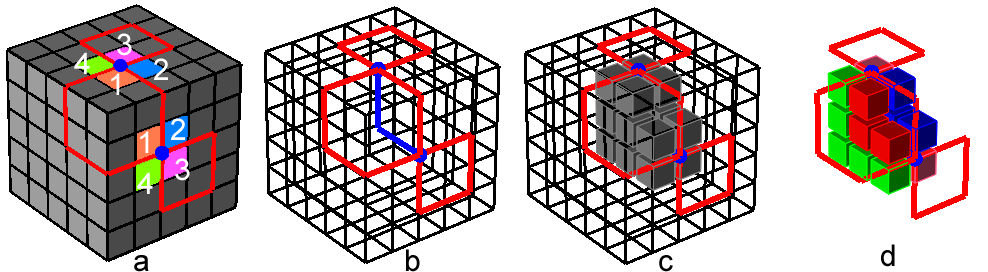
\includegraphics[width=9cm]{det_int_line.png}
\caption{Process of constructing the intersecting line and its int-4-hex-sets: (a) two intersecting nodes paired based on the 1st local intersecting structure; (b) the intersecting line determined by A* algorithm; (c) the hexahedra adjacent to the intersecting line; (d) the int-4-hex-sets of the intersecting line.}
\label{fig:det_int_line}
\end{center}
\end{figure}

%%%%%%%%%%%%%%%%%%%%%%%%%%%%%%%%%%%%%%%%
\subsection{Determination of Initial Quad Set by Max-flow-min-cut Algorithm}
\label{sec:det_init_quad_set}
After constructing the intersecting lines and their int-4-hex-sets, we now construct the initial quad set. The idea is similar to that mentioned in Section \ref{sec:local_separation}, we convert the problem from being able to do local separation to acquiring min cut on a graph. If we see the hexahedra as nodes and the adjacency between the hexahedra as edges of the graph, the quad set is actually a cut set of the graph. Hence, max-flow-min-cut algorithm can be used to efficiently get a quad set that is able to do local separation. This section provides specific details about this process.

As the boundary loop separates the boundary of the local hex set into $2+n$ subsets ($n$ is the number of intersecting nodes), we can get $2+n$ hex sets that are adjacent to these $2+n$ quad sets. From these $2+n$ hex sets and the int-4-hex-sets of the intersecting lines, we merge hex sets that share common hexahedra. This will result in $2+N$ hex sets ($N$ is the number of intersecting lines). We then apply the max-flow-min-cut algorithm multiple times to get the initial quad set. The pseudo-codes are provided in Algorithm \ref{alg:det_init_quad_set}.

\begin{algorithm}
\caption{Determination of the Initial Quad Set}
\label{alg:det_init_quad_set}
\begin{algorithmic}[1]
  \REQUIRE The boundary loop $L$ and the local hex set $H_{local}$;
  \ENSURE The initial quad set $Q_{init}$;
  \STATE $n=$ the count of self-intersecting nodes on $L$;
  \STATE $N=$ the count of intersecting lines;
  \STATE Get the quad subsets on the boundary of $H_{local}$ as $Q_{bound}=\{Q_{b1},Q_{b2},\cdots,Q_{b2+n}\}$;
  \STATE $H_{bound}=\{H_{b1},H_{b2},\cdots,H_{b2+n}\}$ where $H_i$ is the hex set adjacent to $Q_i$,$i=1,2,\cdots,2+n$;
  \STATE $H_{int}=\{H_{in1}^1,H_{in1}^2,H_{in1}^3,H_{in1}^4,\cdots,H_{inN}^1,H_{inN}^2,H_{inN}^3,H_{inN}^4\}$ where $\{H_{ini}^1,H_{ini}^2,H_{ini}^3,H_{ini}^4\}$ is the int-4-hex-sets of the $i$th intersecting line;
  \STATE $H_{merge}=H_{bound} \cup H_{int}$;
  \WHILE{$\exists H_{mi},H_{mj} \in H_{merge}$, $i \neq j$ that $H_{mi} \cap H_{mj} = \emptyset$}
     \STATE Merge $H_{mi}$ and $H_{mj}$;
  \ENDWHILE
  \STATE $Q_{init}=\emptyset$;
  \FOR{each $H_{mi} \in H_{merge}$}
     \STATE $H_{rest}=\bigcup \{H_{merge} - H_{mi}\}$;
     \STATE Let $H_{mi}$ be the $s$ node and $H_{rest}$ be the $j$ node;
     \STATE Perform the max-flow-min-cut algorithm and get the quad set $Q_i$;
     \STATE $Q_{init}=Q_{init} \cup Q_i$;
  \ENDFOR
\end{algorithmic}
\end{algorithm}

Two examples are provided to illustrate the procedures of Algorithm \ref{alg:det_init_quad_set}. The first example is a non-self-intersecting boundary loop as shown in Fig. \ref{fig:non_int_init_qs}. $n$ and $N$ are both 0 for this example. The two quad subsets on the boundary of the local hex set $H$ are $Q_{b1}$ and $Q_{b2}$ as shown in Fig. \ref{fig:non_int_init_qs}(c). We get the two hex sets adjacent to $Q_{b1}$ and $Q_{b2}$ as $H_{b1}$ and $H_{b2}$ (Fig. \ref{fig:non_int_init_qs}(d)). We construct the directed graph by taking $H_{b1}$ as $s$ node and $H_{b2}$ as $t$ node, taking other hexahedra as normal nodes, and assigning weights to the edges according to the number of quads shared by two hex sets. After running the max-flow-min-cut algorithm, we get the initial quad set $Q_{init}$ as shown in Fig. \ref{fig:non_int_init_qs}(e).

\begin{figure}[htbp]
\begin{center}
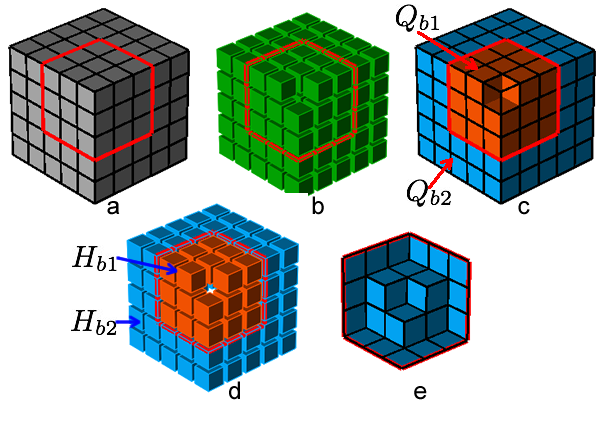
\includegraphics[width=8cm]{non_int_init_qs.png}
\caption{Process of the determination of the initial quad set from a non-intersecting boundary loop: (a) the non-intersecting boundary loop; (b) the local hex set; (c) the two boundary quad subsets $Q_{b1}$(orange) and $Q_{b2}$(blue); (d) two hex sets $H_{b1}$(orange) and $H_{b2}$(blue); (e) the initial quad set $Q_{init}$.}
\label{fig:non_int_init_qs}
\end{center}
\end{figure}

The second example is a self-intersecting boundary loop as shown in Fig. \ref{fig:int_init_qs}. The boundary loop (red in Fig. \ref{fig:int_init_qs}(a)) intersects itself once, hence $n=2,N=1$. We first get the int-4-hex-sets $i4h_1$-$i4h_4$(Fig. \ref{fig:int_init_qs}(b)). The boundary of the local hex set $H$ is separated into $Q_{b1}$-$Q_{b4}$(Fig. \ref{fig:int_init_qs}(c)), and the hex sets adjacent to these quad subsets are $H_{b1}$-$H_{b4}$ (Fig. \ref{fig:int_init_qs}(d) and Fig. \ref{fig:int_init_qs}(e)). Therefore $H_{merge}=H_{int} \cup H_{bound}=\{i4h_1,\cdots,i4h_4,H_{b1},\cdots,H_{b4}\}$. After merging, $H_{merge}=\{H_{m1},H_{m2},H_{m3}\}$ (Fig. \ref{fig:int_init_qs}(f) and Fig. \ref{fig:int_init_qs}(g)). We then conduct the max-flow-min-cut algorithm twice. For the first time, we take $H_{m1}$ as $s$ node and $H_{m2} \cup H_{m3}$ as $t$ node (Fig. \ref{fig:int_init_qs}(h)), and get the quad set $Q_1$ (Fig. \ref{fig:int_init_qs}(i)). For the second time, we take $H_{m2}$ as $s$ node and $H_{m1} \cup H_{m3}$ as $t$ node (Fig. \ref{fig:int_init_qs}(j)), and get the quad set $Q_2$ (Fig. \ref{fig:int_init_qs}(k)). Finally the initial quad set is $Q_{init}=Q_1 \cup Q_2$ (Fig. \ref{fig:int_init_qs}(l)).

\begin{figure*}[htbp]
\begin{center}
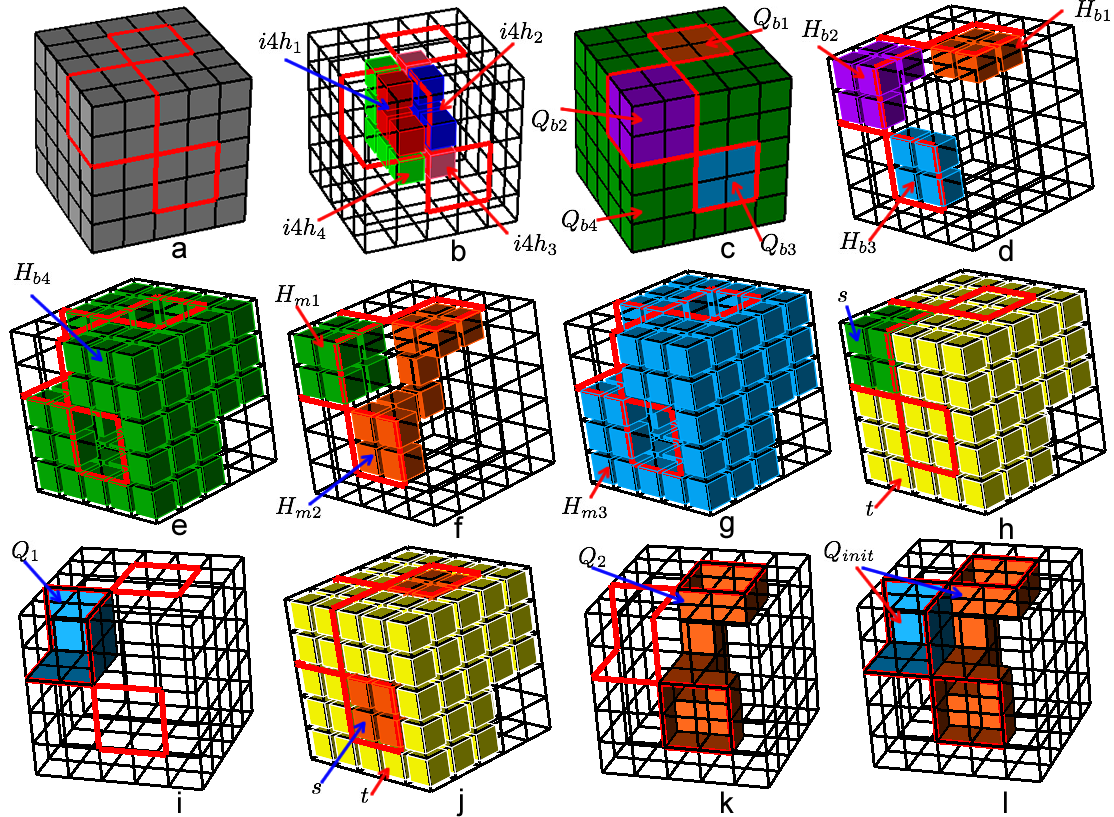
\includegraphics[width=13cm]{int_init_qs.png}
\caption{Process of the determination of the initial quad set from a self-intersecting boundary loop: (a) the self-intersecting boundary loop; (b) the int-4-hex-sets $i4h_1$-$i4h_4$ of the intersecting line; (c) the four quad subsets $Q_{b1}$-$Q_{b4}$ on the boundary of the local hex set separated by the boundary loop; (d) the hex sets $H_{b1}$-$H_{b3}$ adjacent to $Q_{b1}$-$Q_{b3}$ respectively; (e) the hex set $H_{b4}$ adjacent to $Q_{b4}$; (f) the hex set $H_{m1}$ merging from $i4h_1$ and $H_{b2}$ and $H_{m2}$ merging from $i4h_3$, $H_{b1}$ and $H_{b3}$; (g) the hex set $H_{m3}$ merging from $i4h_2$, $i4h_4$ and $H_{b4}$; (h) take $H_{m1}$ as $s$ node and $H_{m2}\cup H_{m3}$ as $t$ node; (i) the quad set $Q_1$ determined by the max-flow-min-cut algorithm; (j) take $H_{m2}$ as $s$ node and $H_{m1} \cup H_{m3}$ as $t$ node; (k) the quad set $Q_2$ determined by the max-flow-min-cut algorithm; (l) the initial quad set $Q_{init}=Q_1 \cup Q_2$.}
\label{fig:int_init_qs}
\end{center}
\end{figure*}

%%%%%%%%%%%%%%%%%%%%%%%%%%%%%%%%%%%%%%%%%%%%%%%%%%%%%%%%%%%%%%%%%%%%%%%%%%
\section{Optimization of the Initial Quad Set}
\label{sec:opt_init_qs}
Although the initial quad set determined by previous section satisfies all the constraints specified by the user, the quality of the mesh after sheet inflation is usually not good enough. In this paper we propose a new optimization method for the quad set based on the quad set's dual structures. In this section we discuss the details of this optimization method.

%%%%%%%%%%%%%%%%%%%%
\subsection{Quality Evaluation of the Quad Set}
\label{sec:quality_eval_qs}
In a hex mesh, the valence of a mesh edge stands for the count of its adjacent quads. Staten et al. showed that the edge valence has direct impact on the mesh quality in \cite{Staten2010d}. For a mesh edge $e$ inside the hex mesh, the ideal valence is 4 because this will make the average dihedral angle at the edge be $90^{\circ}$. When $e$ is on the mesh boundary, however, the ideal valence will be different depending on the dihedral angle $\theta$ between the two boundary quads adjacent to that edge, which can be calculated using Equation \ref{equ:ideal_val}.

\begin{equation}
\label{equ:ideal_val}
IV(e) =
 \begin{cases}
    2 & \text{if $0^{\circ} < \theta \leq 135^{\circ}$,} \\
    3 & \text{if $135^{\circ} < \theta \leq 225^{\circ}$,} \\
    4 & \text{if $225^{\circ} < \theta \leq 315^{\circ}$,} \\
    5 & \text{if $315^{\circ} < \theta < 360^{\circ}$.}
 \end{cases}
\end{equation}

A mesh edge is called a regular edge if its edge valence is ideal. Otherwise it is called an irregular edge. The irregular degree is the difference of valences between one edge and its corresponding regular edge. Suppose $v_e$ stands for a mesh edge $e$'s valence, the irregular degree of $e$ is computed as Equation \ref{equ:irre_deg}.

\begin{equation}
\label{equ:irre_deg}
ID(e) = \left \| v_e-IV(e) \right \|
\end{equation}

Therefore in this paper we use the edges' valences and irregular degree to evaluate the quality of the quad set.

When creating new sheets, different quad sets have different impact on the quality of the mesh. In Fig. \ref{fig:quality_impact_qs}(a), before sheet inflation, $ID(e_1)=0$; after sheet inflation, $e_1$ is splitted into two edges $e_2$ and $e_3$ and $ID(e_2)+ID(e_3)=0$ as shown in Fig. \ref{fig:quality_impact_qs}(c). However, if $Q_2$ (Fig. \ref{fig:quality_impact_qs}(d)) is inflated, although $e_4$ is a regular edge, the two edges splitted from $e_4$ are irregular edges as shown in Fig. \ref{fig:quality_impact_qs}(f), and $ID(e_5)+ID(e_6)=2$. The inherent reason for the difference of irregular degrees is that $Q_1$ and $Q_2$ separate the adjacent hex sets into different configurations as shown in Fig. \ref{fig:quality_impact_qs}(b) and Fig. \ref{fig:quality_impact_qs}(e).

\begin{figure}[htbp]
\begin{center}
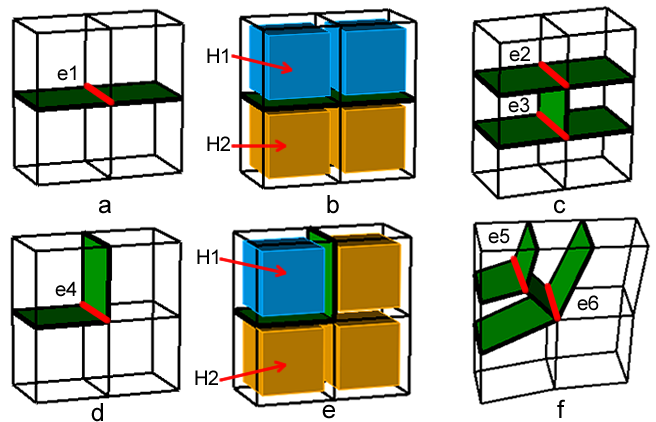
\includegraphics[width=8cm]{quality_impact_qs.png}
\caption{Different impacts on the mesh quality of different quad sets: (a) quad set $Q_1$(green) and one of its mesh edges $e_1$(red); (b) the hex set adjacent to $e_1$ is separated into two subsets $H_1$ and $H_2$ by $Q_1$; (c) $e_1$ is splitted into two edges $e_2$ and $e_3$ after inflation; (d) quad set $Q_2$ and one of its mesh edges $e_4$; (e) the hex set adjacent to $e_4$ is separated into two subsets $H_1$ and $H_2$ by $Q_2$; (f) $e_4$ is splitted into two edges $e_5$ and $e_6$ after inflation.}
\label{fig:quality_impact_qs}
\end{center}
\end{figure}

Suppose $e$ is an edge on quad set $Q$, and $Q$ separates $e$'s adjacent hexahedra into two subsets $H_1$ and $H_2$, and the two new edges created by splitting $e$ are $e'$ and $e''$, then the variation between the irregular degrees of $e$ and two new edges can be computed by Equ. \ref{equ:dif_irre_deg}. $\left \| H_1 \right \|$ and $\left \| H_2 \right \|$ represent the numbers of hexahedra in $H_1$ and $H_2$ respectively. 

\begin{equation}
\label{equ:dif_irre_deg}
\begin{aligned}
\Delta V_e &= ID(e') + ID(e'') - ID(e) \\
&= |\left \| H_1 \right \| + 2 - IV(e')| + |\left \| H_2 \right \| + 2 - IV(e'')| - ID(e)
\end{aligned}
\end{equation}

$IV(e')$ and $IV(e'')$ are usually equal to $IV(e)$ as we try to prevent the quad set from containing mesh edges that reside on the geometric edges in Section \ref{sec:det_init_quad_set}. Therefore, Equ. \ref{equ:dif_irre_deg} can be changed to Equ. \ref{equ:dif_irre_deg_sim} which removes the dependence on the information of the two new edges. This means that we can directly evaluate the quality of the quad set without conducting the real inflation.

\begin{equation}
\label{equ:dif_irre_deg_sim}
\Delta V_e = |\left \| H_1 \right \| + 2 - IV(e)| + |\left \| H_2 \right \| + 2 - IV(e)| - ID(e)
\end{equation}


A negative $\Delta V_e$ means the mesh quality near $e$ has been improved by the inflation, otherwise the mesh quality becomes worse. For example, in Fig. \ref{fig:quality_impact_qs}(d), $IV(e_4)=4$, so $ID(e)=0$. $\left \| H_1 \right \| = 1$ and $\left \| H_2 \right \| = 3$, so $\Delta V_e=|1 + 2 - 4| + |3 + 2 - 4| - 0 = 2$. $\Delta V_e > 0$ means that this inflation makes the mesh quality worse. 

If $Q$ is non-self-intersecting, $E=\{e_1,e_2,\cdots,e_n\}$ is the set of edges on $Q$ where $n$ is the count of the edges, $Q$'s variation of irregular degrees $\Delta V_Q$ can then be computed by Equation \ref{equ:qs_dif_irre_deg}.

\begin{equation}
\label{equ:qs_dif_irre_deg}
\Delta V_Q=\sum_{i=1}^{n}\Delta V_{e_i}
\end{equation}

%%%%%%%%%%%%%%%%%%%%
\subsection{Chord-based Optimization of the Quad Set}
\label{sec:opt_qs_dual}
To improve the quality of the quad set, it needs to adjust the structure of the quad set to make it contain as few edges with large variation of irregular degrees as possible. It is, however, not a trivial task since any changes applied on one edge will inevitably impact its adjacent edges. Theoretically, if we evaluate all the possible quad sets then we can find the optimal quad set with least variation of irregular degrees. Nevertheless it is almost impossible due to the large searching space. Chen et al. proposed an optimization method which locally handles concave or convex edges one by one\cite{Chen:2015kf}. This method avoids the difficulty of global optimization by handling the irregular edges on the quad set in a greedy-based manner. However, it cannot guarantee the mesh quality due to the interaction between edges on the quad set, and sometimes it may be even not convergent. In this paper, we propose an optimization method based on the dual structure of the quad set. Our method not only avoids the difficulty in global optimization, but also guarantees the mesh quality after sheet inflation.

On a quad mesh, starting from an edge, we can recursively get all the edges that are topologically parallel to this edge. These edges and the adjacent quads form a chord, the dual structure of the quad mesh\cite{Murdoch:1997fy,Mitchell1996}. Similar to the quad mesh, the quad set for sheet inflation also consists of chords. All of the mesh edges on the boundary loop pairwise belong to one chord. For example, in Fig. \ref{fig:qs_dual}(b), $e_1$ and $e_2$ belong to the chord $c_1$, and $e_3$ and $e_4$ belong to the chord $c_2$. Theoretically the two kinds of chords, the chord on a quad mesh and the chord on a quad set for sheet inflation, are the same. They are both obtained by recursively searching topologically parallel mesh edges on the quads. The only difference between these two kinds of chords is the chord on a quad mesh is not associated to a sheet (because there are no hexahedra here) while the chord on a quad set for sheet inflation is associated to a sheet (because it resides inside a hex mesh). For example, in Fig. \ref{fig:qs_dual}(c), $e_3$, $e_4$ and their chords are contained in the sheet $s$ (red). Due to the association with a sheet, a chord on the quad set for sheet inflation can be optimized by searching a new path within that sheet to improve the irregular degrees of its edges.

\begin{figure}[htbp]
\begin{center}
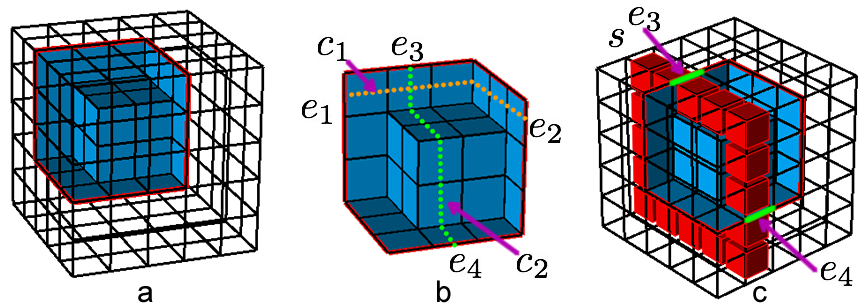
\includegraphics[width=8cm]{qs_dual.png}
\caption{The chords of the quad set: (a) the quad set; (b) two chords $c_1$ and $c_2$ on the quad set; (c) the sheet $s$ that contains $e_3$ and $e_4$.}
\label{fig:qs_dual}
\end{center}
\end{figure}

We improve the quality of the quad set by iteratively improving the quality of the chords that contain the edges on the boundary loop. The chords are neither too constrained as the whole quad set nor too local as one single concave or convex edge. By optimizing the chords, we can effectively improve the quality of the quad set while avoiding the difficulty of optimizing the quad set as a whole. Suppose the quad set is $Q$ and its edge set is $E$, the details of the optimization procedures are explained:

\begin{enumerate}
  \item Divide the edges on the boundary loop into groups according to whether they are in the same sheet. For example, $e_3$ and $e_4$ are grouped in Fig. \ref{fig:qs_opt1}(a), and $e_1$ - $e_4$ are grouped in Fig. \ref{fig:qs_opt2}(a);
  \item Select a group of edges that have not been processed. Get all of the edges in the corresponding sheet and the quads adjacent to these edges. These edges and quads compose the searching space for new chords that connect these edges. Suppose the edge group is $g=\{e_3,e_4\}$, Fig. \ref{fig:qs_opt1}(b) shows the edges that are in the same sheet of $g$ and the adjacent quads;
  \item Since the edges in the group pairwise connect to one chord, we use A* algorithm to search for the new chords. While searching, we take the edges' variation of irregular degrees into consideration. For example, in Fig. \ref{fig:qs_opt1}(c), there are three quads adjacent to $q_1$. If we select $q_2$ or $q_4$ as the next forward step, the variation of irregular degrees of $e_5$ will be 2; if we select $q_3$ as the next forward step, the variation of irregular degrees $e_5$ becomes 0. Hence we select $q_3$. The new chord connecting $e_3$ and $e_4$ is shown in Fig. \ref{fig:qs_opt1}(d). If there are more than two edges in the group, it needs to be decided which two edges should be paired. For example, four edges $e_1$ - $e_4$ in Fig. \ref{fig:qs_opt2}(b) are in the same group. If we connect $e_1$ and $e_3$ and get the new chord $c_3$ (blue in Fig. \ref{fig:qs_opt2}(c)), then $e_2$ and $e_4$ cannot be connected without intersecting with $c_3$ which is not allowed for keeping the quad set valid as shown in Fig. \ref{fig:qs_opt2}(d). So we search new chords between $e_1$ and $e_4$, $e_2$ and $e_3$. The two new chords are shown in Fig. \ref{fig:qs_opt2}(e);
  \item The new chords and the original chords encompass a hex set on the sheet. For example, the hex set $h$ in Fig. \ref{fig:qs_opt1}(e) is encompassed by the two chords $c_2$ an $c_4$, and the hex set $h$ in Fig. \ref{fig:qs_opt2}(f) is encompassed by the four chords $c_1$,$c_2$,$c_4$ and $c_5$. We get the boundary quad set $Q_h$ of $h$, and let $Q$ be the symmetric difference between $Q$ and $Q_h$, i.e. $Q=Q\cup Q_h-Q\cap Q_h$. The updated $Q$ is shown in Fig. \ref{fig:qs_opt1}(f) and Fig. \ref{fig:qs_opt1}(g);
  \item Repeat the process of Step 2-4 until all of the edge groups are handled. The final quad sets for the two examples are shown in Fig. \ref{fig:qs_opt1}(g) and Fig. \ref{fig:qs_opt2}(g).
\end{enumerate}

\begin{figure}[htbp]
\begin{center}
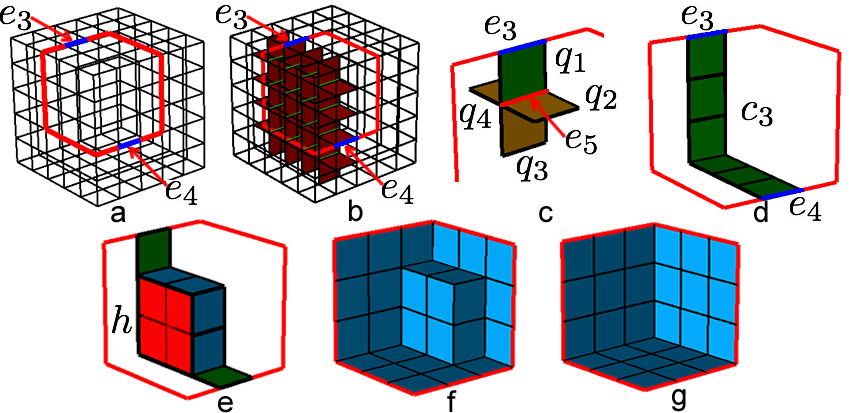
\includegraphics[width=8cm]{qs_opt1.png}
\caption{The 1st example of the quad set optimization: (a) two edges $e_3$ and $e_4$ on the boundary loop; (b) the edges on the sheet (green) and adjacent quads (red); (c) $q_1$'s three adjacent quads $q_2$, $q_3$ and $q_4$; (d) the new chord connecting $e_3$ and $e_4$; (e) the hex set $h$ encompassed by the two chords; (f) $Q$ is updated by getting the symmetric difference between $Q$ and $Q_h$; (g) the final quad set.}
\label{fig:qs_opt1}
\end{center}
\end{figure}

The variation of irregular degrees $\Delta V_Q$ of the initial quad set in Fig. \ref{fig:qs_dual}(a) is 42. After optimization, the variation of irregular degrees of the quad set in Fig. \ref{fig:qs_opt1}(g) $\Delta V_Q'$ becomes 18, which is 24 smaller than $\Delta V_Q$.

\begin{figure}[htbp]
\begin{center}
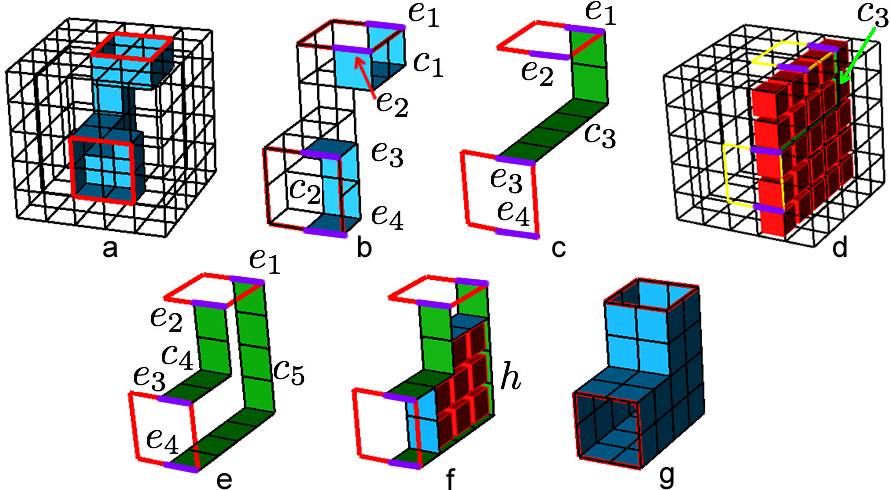
\includegraphics[width=8cm]{qs_opt2.png}
\caption{The 2nd example of the quad set optimization: (a) the initial quad set; (b) $e_1$-$e_4$ on the same sheet and two chords $c_1$ and $c_2$; (c) the new chord $c_3$ connecting $e_1$ and $e_3$; (d) $e_2$ and $e_4$ cannot be connected by a chord without intersecting $c_3$; (e) the two new chords $c_4$ and $c_5$; (f) the hex set $h$ encompassed by the four chords; (g) $Q$ is updated by getting the symmetric difference between $Q$ and $Q_h$.}
\label{fig:qs_opt2}
\end{center}
\end{figure}

The variation of irregular degrees $\Delta V_Q$ of the initial quad set in Fig. \ref{fig:qs_opt2}(a) is 76, and it becomes 56 after optimization which is 20 smaller.

If the quad set is self-intersecting, we first split it into quad subsets at the intersecting line. For example, in Fig. \ref{fig:opt_int_quad_sets}, we separate the quad set into $QS_1$ and $QS_2$ (Fig. \ref{fig:opt_int_quad_sets}(b)). Then we apply the above optimization algorithm on these quad subsets separately. The quads adjacent to the intersecting line(Fig. \ref{fig:opt_int_quad_sets}(c)) should keep unchanged in order to keep the topology valid.

\begin{figure}[htbp]
\begin{center}
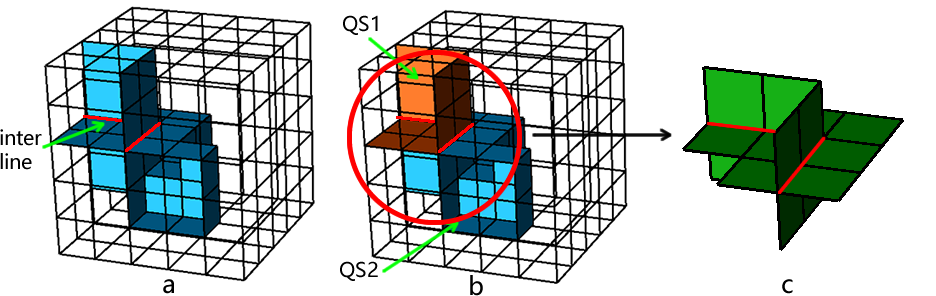
\includegraphics[width=8cm]{opt_int_quad_sets.png}
\caption{Optimization of the self-intersecting quad set: (a) the self-intersecting quad set with the intersecting line(red); (b) we first separate it into individual quad subsets and then conduct the optimization algorithm on them successively; (c) the quads adjacent to the intersecting line should be kept unchanged.}
\label{fig:opt_int_quad_sets}
\end{center}
\end{figure}

%%%%%%%%%%%%%%%%%%%%%%%%%%%%%%%%%%%%%%%%%%%%%%%%%%%%%%%%%%%%%%%%%%%%%%%%%%
\section{Examples}
\label{sec:examples}
We implement our approach in C++ on a 32-bit Windows 7 platform, using Visual Studio 2010. The approach has been tested on different meshes under various constraints. This section presents three practical applications of the approach: one is complex sheets generation for mesh matching and the other two are the quality improvement for the mesh boundary by reducing high node valences. In these three examples, self-intersecting sheets are all required to be locally generated. Comparisons between our approach and existing works are also provided at the end of this section.

%%%%%%%%%%%%%%%%%%%%%%%%%%%%%%%%%%%%%%%%
\subsection{Complex Sheets Generation for Mesh Matching}
\label{sec:mesh_matching}
Mesh matching is an algorithm to convert non-conforming interfaces to conforming ones\cite{Chen:2015kf,Staten2010d}. Starting from interfaces with different topologies, it gradually changes the interfaces' topologies by sheet operations until the interfaces' topologies become identical. The typical process of the mesh matching algorithm is shown in Fig. \ref{fig:mesh_matching_exam}.

\begin{figure*}[htbp]
\begin{center}
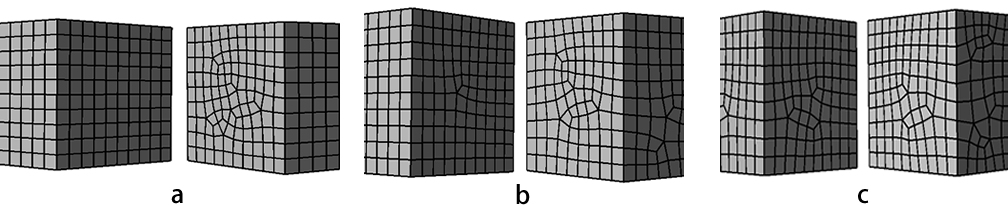
\includegraphics[width=16.5cm]{mesh_matching.png}
\caption{The typical process of mesh matching: (a) non-conformal interfaces; (b) interfaces are changed by sheet operations; (c) non-conformal interfaces are converted to conformal interfaces.}
\label{fig:mesh_matching_exam}
\end{center}
\end{figure*}

Our approach in this paper can be used in mesh matching to locally generate complex sheets that intersect themselves multiple times, which cannot be done in these previous works. In Fig. \ref{fig:exam1_input}, there is an unmatched chord on the interface of hex mesh $M_a$ in Fig. \ref{fig:exam1_input}(b). A new sheet needs to be created to match it on hex mesh $M_b$ under the constraints shown in Fig. \ref{fig:exam1_input}a ($H$ is the volumetric constraints).

\begin{figure}[htbp]
\begin{center}
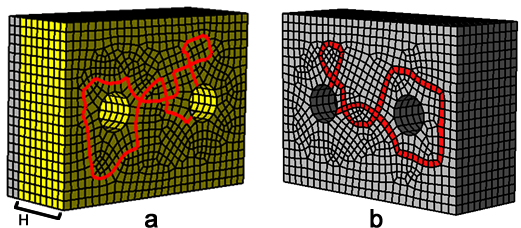
\includegraphics[width=8cm]{exam1_input.png}
\caption{Complex sheet inflation is needed for mesh matching: (a) the constraints for sheet inflation on mesh $M_a$; (b) the unmatched chord(red) on mesh $M_b$.}
\label{fig:exam1_input}
\end{center}
\end{figure}

Under the constraints, we construct the boundary loop as shown in Fig. \ref{fig:exam1_bound_loop}. Since the constraint edges contain three intersecting nodes, a new intersecting node is created as shown in Fig. \ref{fig:exam1_bound_loop}(b). By running the max-flow-min-cut algorithm, new edges are found, enabling the boundary loop to do local separation. The final boundary loop is shown in Fig. \ref{fig:exam1_bound_loop}(e).

\begin{figure}[htbp]
\begin{center}
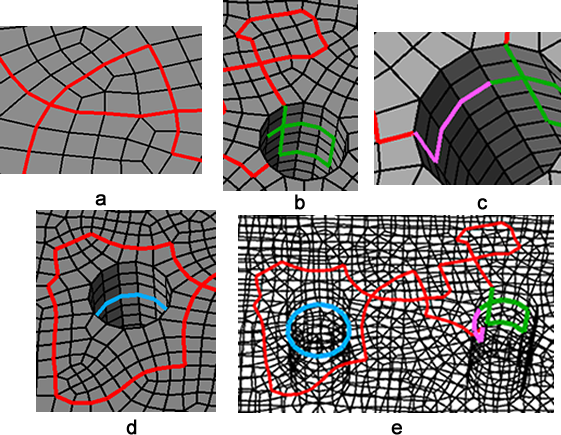
\includegraphics[width=8cm]{exam1_bound_loop.png}
\caption{Determination of the boundary loop: (a) the two intersecting nodes are paired; (b) a new intersecting node is created; (c) the boundary loop is closed; (d) new edges are determined by the max-flow-min-cut algorithm; (e) the final boundary loop.}
\label{fig:exam1_bound_loop}
\end{center}
\end{figure}

Intersecting lines are then constructed, as well as the int-4-hex-sets as shown in Fig. \ref{fig:exam1_quad_set}(a) and Fig. \ref{fig:exam1_quad_set}(b). Then we get the merged hex sets in Fig. \ref{fig:exam1_quad_set}(c) and the initial quad set in Fig. \ref{fig:exam1_quad_set}(d). The variation of irregular degrees of the initial quad set is 478. By contrast, the final quad set is much better after optimization as shown in Fig. \ref{fig:exam1_quad_set}(e) whose variation of irregular degrees is reduced to 351.

\begin{figure}[htbp]
\begin{center}
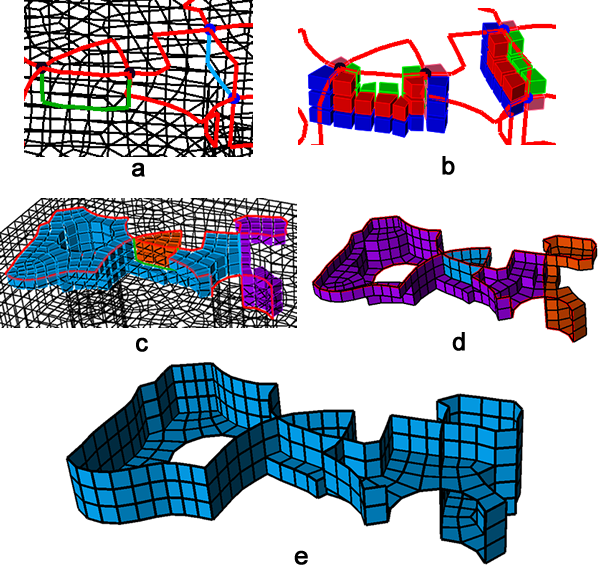
\includegraphics[width=8cm]{exam1_quad_set.png}
\caption{Determination of the quad set: (a) constructing the intersecting lines; (b) the int-4-hex-sets; (c) the merged hex sets; (d) the initial quad set; (e) the optimized quad set.}
\label{fig:exam1_quad_set}
\end{center}
\end{figure}

The new sheet is inflated from the quad set as shown in Fig. \ref{fig:exam1_sheet}.

\begin{figure}[htbp]
\begin{center}
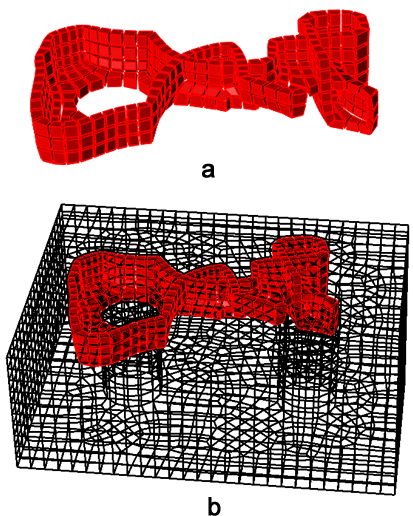
\includegraphics[width=6cm]{exam1_sheet.png}
\caption{Sheet inflation: (a) the new sheet inflated from the quad set; (b) the new sheet in the hex mesh.}
\label{fig:exam1_sheet}
\end{center}
\end{figure}

%%%%%%%%%%%%%%%%%%%%%%%%%%%%%%%%%%%%%%%%
\subsection{High Edge Valences Reduction}
\label{sec:red_edge_val}
In hex meshes, the elements in the area near the boundary are usually very important for finite element analysis\cite{Kowalski2011}. Meanwhile, the node valence and edge valence are critical for the quality of the quad mesh and hex mesh respectively\cite{Owen1998, Staten2010d,Tarini2010}. High node valence or edge valence will largely reduce the accuracy and efficiency of the analysis, or even make the mesh unable to be handled by the solver. The fun sheet matching algorithm proposed by Kowalski et al. \cite{Kowalski2011} can help the hex mesh capture the geometric boundary by inserting fundamental sheets. This algorithm, however, can neither improve the node valences on the mesh boundary nor the edge valence near the mesh boundary. In this section, we present two examples to show how our approach can be used to reduce the high node valences and edge valences near the mesh boundary.

Figure \ref{fig:exam2_input}(a) shows a hex mesh that contains two boundary nodes $v_1$ and $v_2$ with high valences. The valences of $v_1$ and $v_2$ are 6 and 7 respectively. Consequently, the edges inside the hex mesh that are adjacent to these two nodes also have high valences which are 6 and 7 respectively as shown in Fig. \ref{fig:exam2_input}(b). It is usually unacceptable for node or edge valences to be larger than 5 near the boundary. Therefore, these high valences need to be reduced.

\begin{figure}[htbp]
\begin{center}
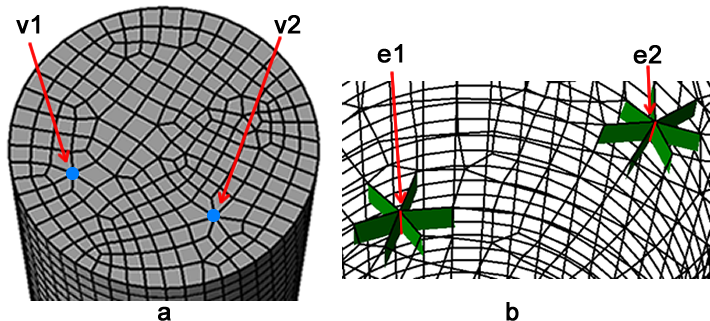
\includegraphics[width=8cm]{exam2_input.png}
\caption{Nodes and edges with high valences: (a) $v_1$'s valence is 6 and $v_2$'s valence is 7; (b) $v_1$'s adjacent edge $e_1$ has the valence of 6 and $v_2$'s adjacent edge $e_2$ has the valence of 7.}
\label{fig:exam2_input}
\end{center}
\end{figure}

To reduce the high valences by our approach, the user first select several edges on the mesh boundary that are adjacent to the two nodes and the local region as shown in Fig. \ref{fig:exam2_bound_loop}(a). Our approach takes these edges as constraints, and then try to achieve the sheet inflation under the constraints. Figure \ref{fig:exam2_bound_loop}(b) and Fig. \ref{fig:exam2_bound_loop}(c) show the process of determination of the boundary loop, and the final boundary loop is shown in Fig. \ref{fig:exam2_bound_loop}(d).

\begin{figure}[htbp]
\begin{center}
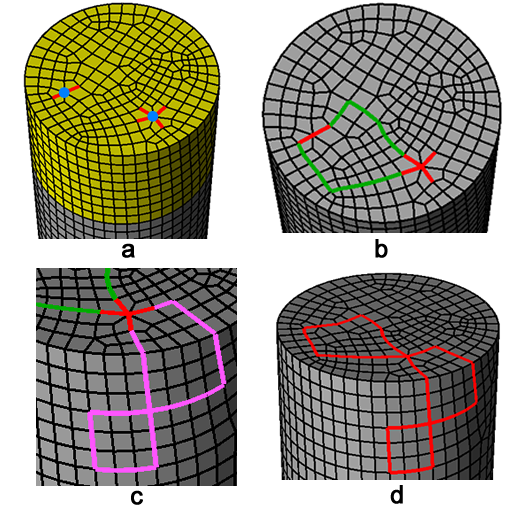
\includegraphics[width=8cm]{exam2_bound_loop.png}
\caption{User-specified constraints and the determination of the boundary loop: (a) several boundary edges adjacent to $v_1$ and $v_2$ are selected as boundary constraints(red) and a set of hexahedra are selected as local region (yellow); (b) the constraint edges are first connected; (c) a new intersecting node is created; (d) the final boundary loop.}
\label{fig:exam2_bound_loop}
\end{center}
\end{figure}

The quad set is then constructed through the procedures shown in Fig. \ref{fig:exam2_quad_set}. The variation of irregular degrees of the initial quad set is 184. The final optimized quad set is shown in Fig. \ref{fig:exam2_quad_set}(e) and its variation of irregular degrees is reduced to 159.

\begin{figure}[htbp]
\begin{center}
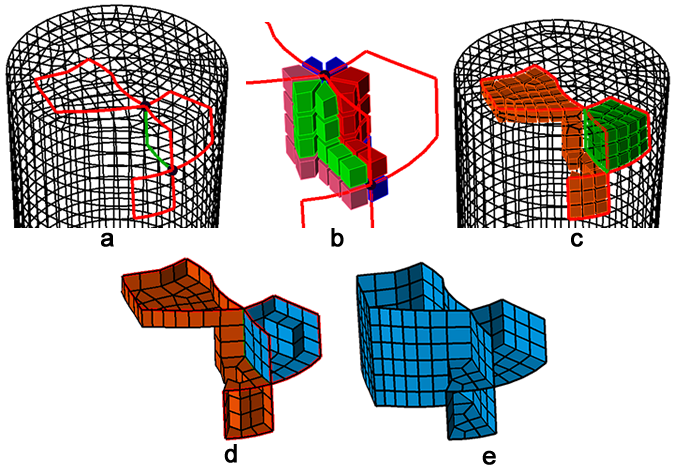
\includegraphics[width=8cm]{exam2_quad_set.png}
\caption{Process of the determination of the quad set: (a) the intersecting line is determined; (b) the int-4-hex-sets are constructed; (c) the merged hex sets; (d) the initial quad set; (e) the optimized quad set.}
\label{fig:exam2_quad_set}
\end{center}
\end{figure}

Sheet inflation is conducted after getting the quad set. The new sheet is shown in Fig \ref{fig:exam2_sheet}(a) and Fig. \ref{fig:exam2_sheet}(b). The two nodes $v_1$ and $v_2$ are actually splitted into two nodes and four nodes respectively as shown in Fig. \ref{fig:exam2_sheet}(c). The new edges splitted from $e_1$ and $e_2$ are shown in Fig. \ref{fig:exam2_sheet}(b). There has no longer any nodes or edges with valences larger than 5.

\begin{figure}[htbp]
\begin{center}
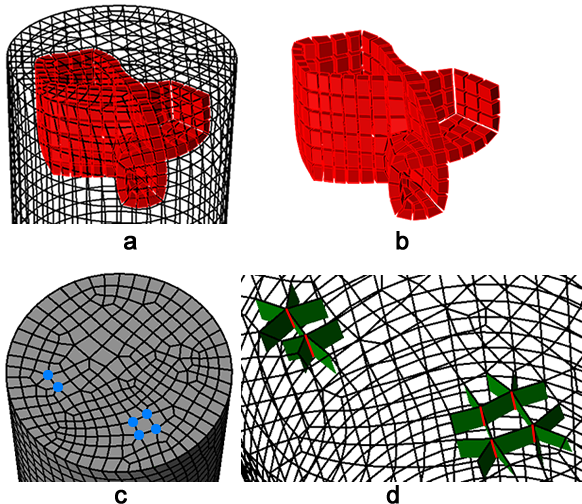
\includegraphics[width=8cm]{exam2_sheet.png}
\caption{Results of high valences reduction: (a) the new sheet inflated from the quad set in the hex mesh; (b) the new sheet; (c) the new nodes with valences no larger than 5; (d) new edges with valences no larger than 5.}
\label{fig:exam2_sheet}
\end{center}
\end{figure}

We have also tested our algorithm with the famous Stanford Bunny. As shown in Fig. \ref{fig:bunny_input}, the hex mesh of Stanford Bunny contains two high-valence boundary nodes. To reduce the valences of these two nodes, a sheet inflation is conducted, creating a self-intersecting sheet. The major steps are shown in Fig. \ref{fig:bunny_proc}. And the modification result is shown in Fig. \ref{fig:bunny_result}, where  the high valences of the two nodes are successfully reduced.

\begin{figure}[htbp]
\begin{center}
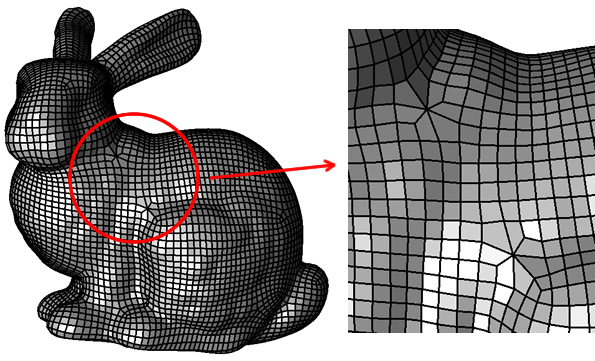
\includegraphics[width=8cm]{bunny_input.png}
\caption{Hex mesh of Stanford Bunny with two high-valence boundary nodes.}
\label{fig:bunny_input}
\end{center}
\end{figure}


\begin{figure}[htbp]
\begin{center}
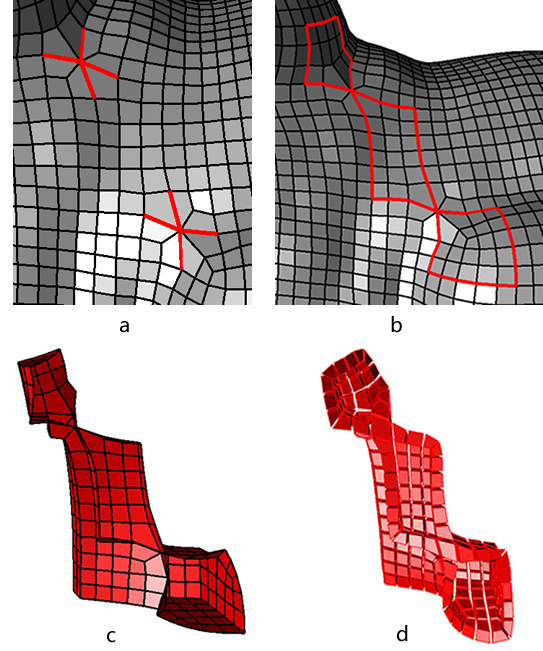
\includegraphics[width=8cm]{bunny_proc.png}
\caption{Process of reducing the high node valences on Stanford Bunny: (a) several boundary edges adjacent to the high-valence nodes are selected as boundary constraints; (b) the boundary loop is constructed; (c) the quad set is constructed; (d) the new sheet is inflated.}
\label{fig:bunny_proc}
\end{center}
\end{figure}

\begin{figure}[htbp]
\begin{center}
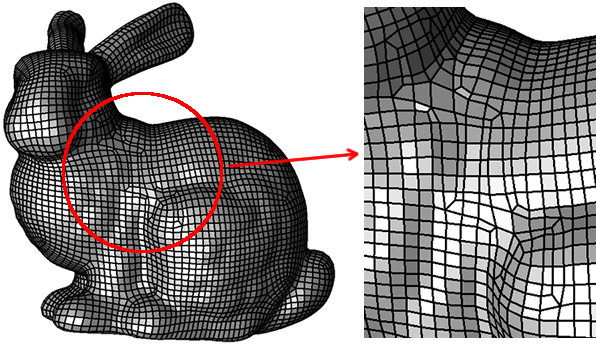
\includegraphics[width=8cm]{bunny_result.png}
\caption{The high node valences are reduced by conducting our sheet inflation.}
\label{fig:bunny_result}
\end{center}
\end{figure}

\subsection{Comparisons with existing works}
\label{sec:comparisons}
Results show that our approach can effectively generate complex localized sheets that self-intersect more than once while guaranteeing the mesh quality. Comparisons are made between our approach and existing works including Mitchell's Pillowing\cite{Mitchell:1995wa}, Staten's General Sheet Inflation\cite{Staten:2009bo} and Chen's Sheet Inflation\cite{Chen:2015kf}. Table \ref{tab:comparisons} lists the detailed comparisons between our approach and existing works.

% Requires the booktabs if the memoir class is not being used
\begin{table*}[htbp]

\caption{Comparisons with existing works.}
\centering
\label{tab:comparisons}
\begin{tabular}{lccc}
\hline
                                                                           & Example 1 (Mesh Matching)                                                                & Example 2 (Valences Reduction in cylinder)                                                                 & Example 3 (Stanford Bunny)                                                 \\ \hline
Mitchell's Pillowing                                                       & \multicolumn{3}{c}{Does not support self-intersecting sheets}                                                                                                                                                                       \\ \hline
\begin{tabular}[c]{@{}l@{}}Staten's\\ General Sheet Inflation\end{tabular} & \multicolumn{3}{c}{Insufficient details to implement}                                                                                                                                                                               \\ \hline
Chen's Sheet Inflation                                                     & Failed                                                                    & \begin{tabular}[c]{@{}c@{}}Succeed.\\ Irregular degrees = 177\end{tabular} & \begin{tabular}[c]{@{}c@{}}Succeed.\\ Irregular degrees = 285\end{tabular} \\ \hline
Our Sheet Inflation                                                        & \begin{tabular}[c]{@{}c@{}}Succeed.\\ Irregular degrees =351\end{tabular} & \begin{tabular}[c]{@{}c@{}}Succeed.\\ Irregular degrees = 159\end{tabular} & \begin{tabular}[c]{@{}c@{}}Succeed.\\ Irregular degrees = 196\end{tabular} \\ \hline
\end{tabular}
\end{table*}

Pillowing cannot handle these three examples because it does not support self-intersecting sheets. And Staten provides insufficient details to implement. Although Chen's Sheet Inflation can inflate sheets that self-intersect only once, the mesh quality suffers from their optimization algorithm due to the fact that their optimization algorithm is based on simply handling concave/convex mesh edges. Our approach can achieve better mesh quality thanks to the new chord-based optimization algorithm.

%%%%%%%%%%%%%%%%%%%%%%%%%%%%%%%%%%%%%%%%%%%%%%%%%%%%%%%%%%%%%%%%%%%%%%%%%%
\section{Conclusions and Future Work}
In this paper, a new approach is proposed to achieving optimized complex sheet inflation under various constraints. Main features of our approach are summarized:

\begin{enumerate}
  \item By using the A* and the max-flow-min-cut algorithms, the valid boundary loop of the quad set for sheet inflation is effectively determined, which satisfies the boundary constraints.
  \item With intersecting nodes on the boundary loop being reasonably paired by recursively searching two local intersecting structures, valid intersecting lines are constructed between each pair of nodes by using A* algorithm, and the int-4-hex-sets are determined around the intersecting lines, enabling our approach to effectively construct complex quad sets that intersect themselves more than once.
  \item By using max-flow-min-cut algorithm, the valid initial quad set is effectively and efficiently determined within the local region specified by the user.
  \item A chord-based optimization method is proposed which can effectively improve the quality of the quad set while avoiding the difficulty in optimizing the quad set as a whole.
\end{enumerate}

Compared with previous sheet inflation methods, three examples show that our approach can effectively generate complex sheets within a local region while guaranteeing the mesh quality. These three examples also present two applications that our approach can be used: one is modifying the interfaces in mesh matching and the other is reducing node valences and edge valences to improve mesh quality.

The shortcomings of our approach and future work are listed below:
\begin{enumerate}
  \item It is not very convenient to generate self-touching sheets. In some rare cases, self-touching sheets need to be generated. By combining other dual operations like column collapse and sheet extraction, our approach is able to create self-touching sheets. However, currently it is not very convenient. We will propose simpler solutions to generate self-touching sheets;
  \item Currently the constraints can only be specified by boundary edges and hexahedra. However, sometimes the user needs to specify edges or quads inside the hex mesh to control the sheet inflation, e.g. improving the edge valences inside the hex mesh. Hence, we plan to adapt our approach to accept constraints specified inside the hex mesh.
\end{enumerate}

\section*{Acknowledgements}
The authors are very grateful to the financial supports from NSF of China (61572432) and National 863 High Technology Plan (2013AA041301).

\section*{References}
\bibliographystyle{model3-num-names}
\bibliography{ref}

\end{document}
